\documentclass[1p]{elsarticle_modified}
%\bibliographystyle{elsarticle-num}

%\usepackage[colorlinks]{hyperref}
%\usepackage{abbrmath_seonhwa} %\Abb, \Ascr, \Acal ,\Abf, \Afrak
\usepackage{amsfonts}
\usepackage{amssymb}
\usepackage{amsmath}
\usepackage{amsthm}
\usepackage{scalefnt}
\usepackage{amsbsy}
\usepackage{kotex}
\usepackage{caption}
\usepackage{subfig}
\usepackage{color}
\usepackage{graphicx}
\usepackage{xcolor} %% white, black, red, green, blue, cyan, magenta, yellow
\usepackage{float}
\usepackage{setspace}
\usepackage{hyperref}

\usepackage{tikz}
\usetikzlibrary{arrows}

\usepackage{multirow}
\usepackage{array} % fixed length table
\usepackage{hhline}

%%%%%%%%%%%%%%%%%%%%%
\makeatletter
\renewcommand*\env@matrix[1][\arraystretch]{%
	\edef\arraystretch{#1}%
	\hskip -\arraycolsep
	\let\@ifnextchar\new@ifnextchar
	\array{*\c@MaxMatrixCols c}}
\makeatother %https://tex.stackexchange.com/questions/14071/how-can-i-increase-the-line-spacing-in-a-matrix
%%%%%%%%%%%%%%%

\usepackage[normalem]{ulem}

\newcommand{\msout}[1]{\ifmmode\text{\sout{\ensuremath{#1}}}\else\sout{#1}\fi}
%SOURCE: \msout is \stkout macro in https://tex.stackexchange.com/questions/20609/strikeout-in-math-mode

\newcommand{\cancel}[1]{
	\ifmmode
	{\color{red}\msout{#1}}
	\else
	{\color{red}\sout{#1}}
	\fi
}

\newcommand{\add}[1]{
	{\color{blue}\uwave{#1}}
}

\newcommand{\replace}[2]{
	\ifmmode
	{\color{red}\msout{#1}}{\color{blue}\uwave{#2}}
	\else
	{\color{red}\sout{#1}}{\color{blue}\uwave{#2}}
	\fi
}

\newcommand{\Sol}{\mathcal{S}} %segment
\newcommand{\D}{D} %diagram
\newcommand{\A}{\mathcal{A}} %arc


%%%%%%%%%%%%%%%%%%%%%%%%%%%%%5 test

\def\sl{\operatorname{\textup{SL}}(2,\Cbb)}
\def\psl{\operatorname{\textup{PSL}}(2,\Cbb)}
\def\quan{\mkern 1mu \triangleright \mkern 1mu}

\theoremstyle{definition}
\newtheorem{thm}{Theorem}[section]
\newtheorem{prop}[thm]{Proposition}
\newtheorem{lem}[thm]{Lemma}
\newtheorem{ques}[thm]{Question}
\newtheorem{cor}[thm]{Corollary}
\newtheorem{defn}[thm]{Definition}
\newtheorem{exam}[thm]{Example}
\newtheorem{rmk}[thm]{Remark}
\newtheorem{alg}[thm]{Algorithm}

\newcommand{\I}{\sqrt{-1}}
\begin{document}

%\begin{frontmatter}
%
%\title{Boundary parabolic representations of knots up to 8 crossings}
%
%%% Group authors per affiliation:
%\author{Yunhi Cho} 
%\address{Department of Mathematics, University of Seoul, Seoul, Korea}
%\ead{yhcho@uos.ac.kr}
%
%
%\author{Seonhwa Kim} %\fnref{s_kim}}
%\address{Center for Geometry and Physics, Institute for Basic Science, Pohang, 37673, Korea}
%\ead{ryeona17@ibs.re.kr}
%
%\author{Hyuk Kim}
%\address{Department of Mathematical Sciences, Seoul National University, Seoul 08826, Korea}
%\ead{hyukkim@snu.ac.kr}
%
%\author{Seokbeom Yoon}
%\address{Department of Mathematical Sciences, Seoul National University, Seoul, 08826,  Korea}
%\ead{sbyoon15@snu.ac.kr}
%
%\begin{abstract}
%We find all boundary parabolic representation of knots up to 8 crossings.
%
%\end{abstract}
%\begin{keyword}
%    \MSC[2010] 57M25 
%\end{keyword}
%
%\end{frontmatter}

%\linenumbers
%\tableofcontents
%
\newcommand\colored[1]{\textcolor{white}{\rule[-0.35ex]{0.8em}{1.4ex}}\kern-0.8em\color{red} #1}%
%\newcommand\colored[1]{\textcolor{white}{ #1}\kern-2.17ex	\textcolor{white}{ #1}\kern-1.81ex	\textcolor{white}{ #1}\kern-2.15ex\color{red}#1	}

{\Large $\underline{12n_{0839}~(K12n_{0839})}$}

\setlength{\tabcolsep}{10pt}
\renewcommand{\arraystretch}{1.6}
\vspace{1cm}\begin{tabular}{m{100pt}>{\centering\arraybackslash}m{274pt}}
\multirow{5}{120pt}{
	\centering
	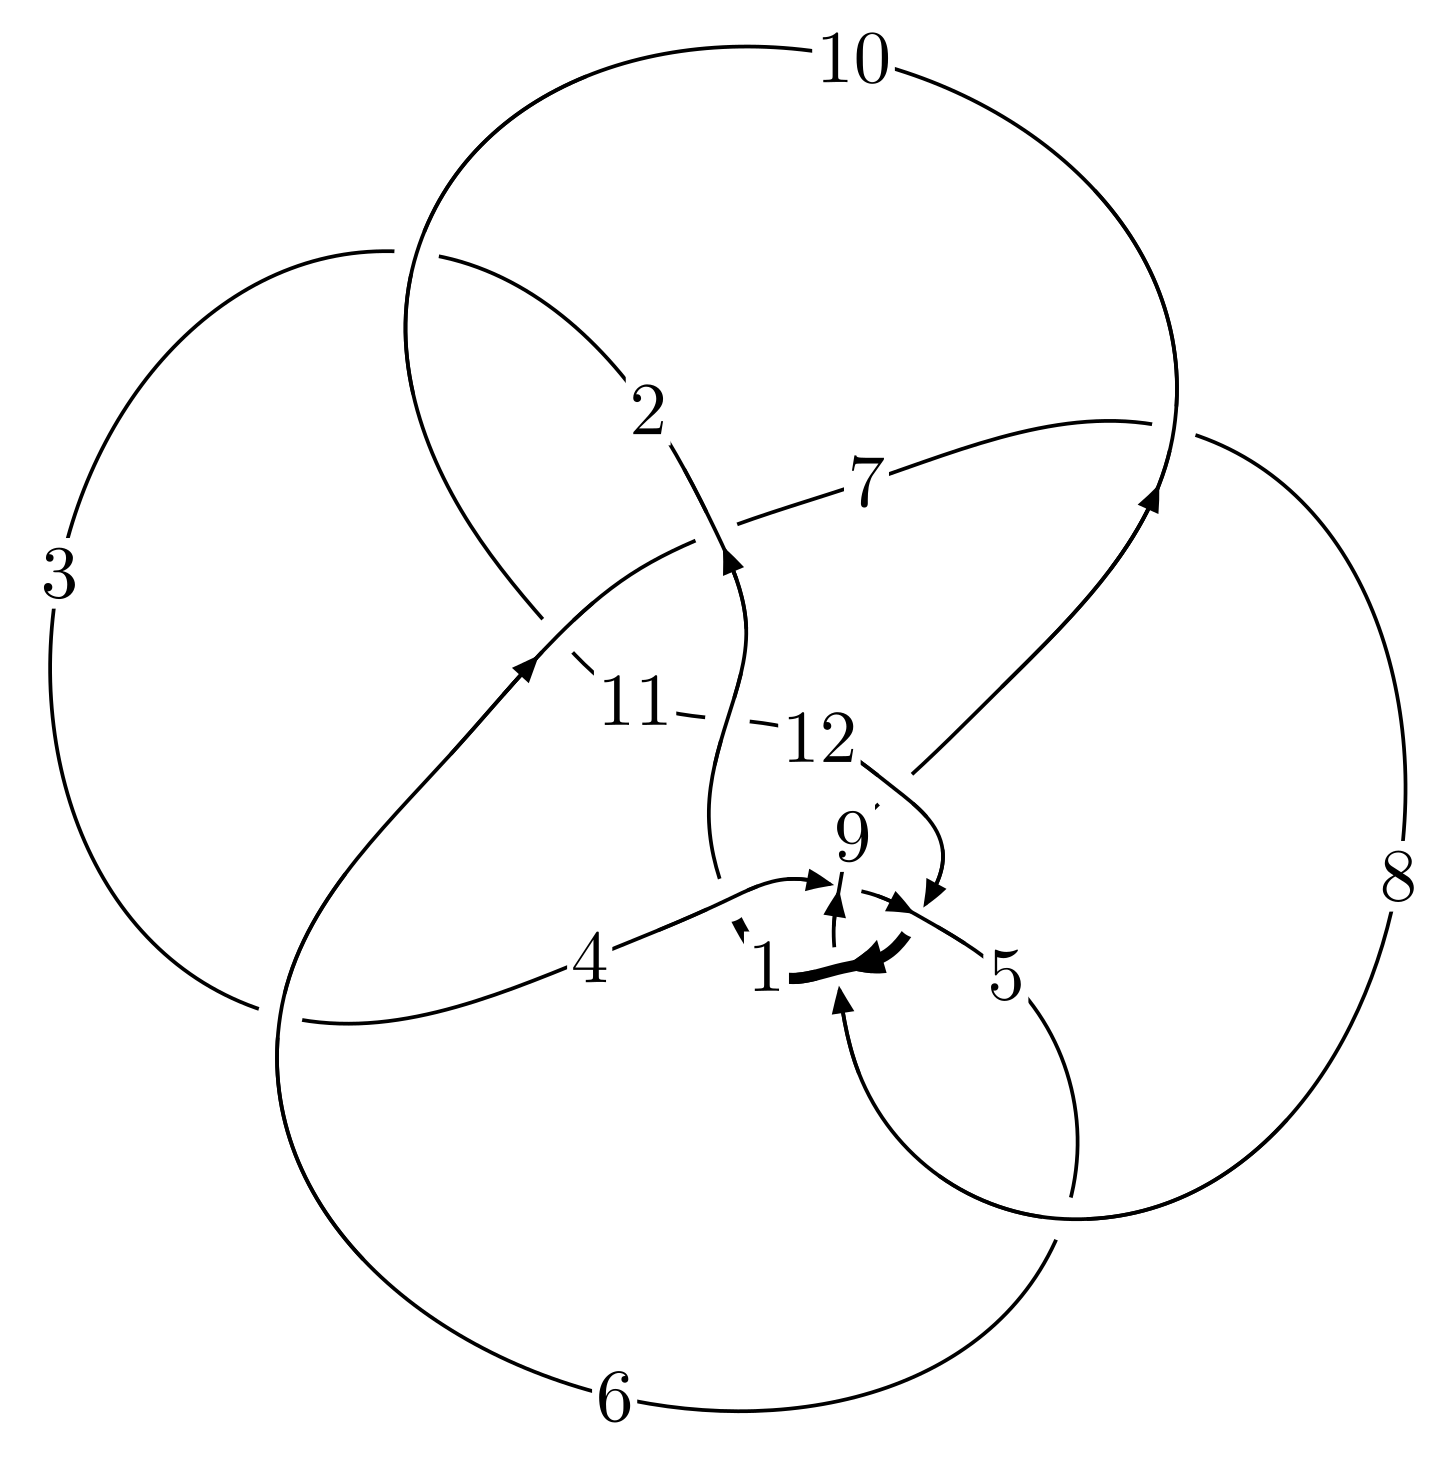
\includegraphics[width=112pt]{../../../GIT/diagram.site/Diagrams/png/2928_12n_0839.png}\\
\ \ \ A knot diagram\footnotemark}&
\allowdisplaybreaks
\textbf{Linearized knot diagam} \\
\cline{2-2}
 &
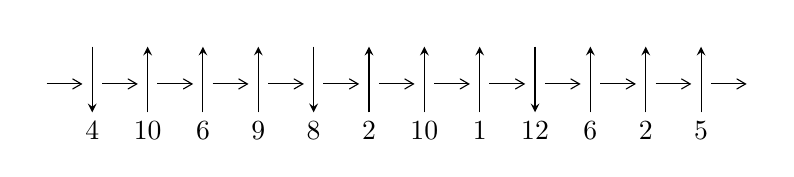
\begin{tikzpicture}[x=20pt, y=17pt]
	% nodes
	\node (C0) at (0, 0) {};
	\node (C1) at (1, 0) {};
	\node (C1U) at (1, +1) {};
	\node (C1D) at (1, -1) {4};

	\node (C2) at (2, 0) {};
	\node (C2U) at (2, +1) {};
	\node (C2D) at (2, -1) {10};

	\node (C3) at (3, 0) {};
	\node (C3U) at (3, +1) {};
	\node (C3D) at (3, -1) {6};

	\node (C4) at (4, 0) {};
	\node (C4U) at (4, +1) {};
	\node (C4D) at (4, -1) {9};

	\node (C5) at (5, 0) {};
	\node (C5U) at (5, +1) {};
	\node (C5D) at (5, -1) {8};

	\node (C6) at (6, 0) {};
	\node (C6U) at (6, +1) {};
	\node (C6D) at (6, -1) {2};

	\node (C7) at (7, 0) {};
	\node (C7U) at (7, +1) {};
	\node (C7D) at (7, -1) {10};

	\node (C8) at (8, 0) {};
	\node (C8U) at (8, +1) {};
	\node (C8D) at (8, -1) {1};

	\node (C9) at (9, 0) {};
	\node (C9U) at (9, +1) {};
	\node (C9D) at (9, -1) {12};

	\node (C10) at (10, 0) {};
	\node (C10U) at (10, +1) {};
	\node (C10D) at (10, -1) {6};

	\node (C11) at (11, 0) {};
	\node (C11U) at (11, +1) {};
	\node (C11D) at (11, -1) {2};

	\node (C12) at (12, 0) {};
	\node (C12U) at (12, +1) {};
	\node (C12D) at (12, -1) {5};
	\node (C13) at (13, 0) {};

	% arrows
	\draw[->,>={angle 60}]
	(C0) edge (C1) (C1) edge (C2) (C2) edge (C3) (C3) edge (C4) (C4) edge (C5) (C5) edge (C6) (C6) edge (C7) (C7) edge (C8) (C8) edge (C9) (C9) edge (C10) (C10) edge (C11) (C11) edge (C12) (C12) edge (C13) ;	\draw[->,>=stealth]
	(C1U) edge (C1D) (C2D) edge (C2U) (C3D) edge (C3U) (C4D) edge (C4U) (C5U) edge (C5D) (C6D) edge (C6U) (C7D) edge (C7U) (C8D) edge (C8U) (C9U) edge (C9D) (C10D) edge (C10U) (C11D) edge (C11U) (C12D) edge (C12U) ;
	\end{tikzpicture} \\
\hhline{~~} \\& 
\textbf{Solving Sequence} \\ \cline{2-2} 
 &
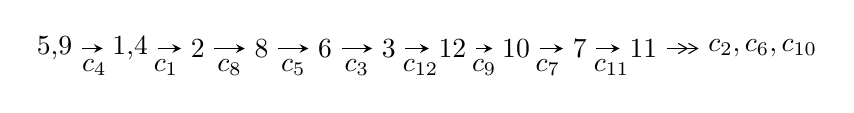
\begin{tikzpicture}[x=23pt, y=7pt]
	% node
	\node (A0) at (-1/8, 0) {5,9};
	\node (A1) at (17/16, 0) {1,4};
	\node (A2) at (17/8, 0) {2};
	\node (A3) at (25/8, 0) {8};
	\node (A4) at (33/8, 0) {6};
	\node (A5) at (41/8, 0) {3};
	\node (A6) at (49/8, 0) {12};
	\node (A7) at (57/8, 0) {10};
	\node (A8) at (65/8, 0) {7};
	\node (A9) at (73/8, 0) {11};
	\node (C1) at (1/2, -1) {$c_{4}$};
	\node (C2) at (13/8, -1) {$c_{1}$};
	\node (C3) at (21/8, -1) {$c_{8}$};
	\node (C4) at (29/8, -1) {$c_{5}$};
	\node (C5) at (37/8, -1) {$c_{3}$};
	\node (C6) at (45/8, -1) {$c_{12}$};
	\node (C7) at (53/8, -1) {$c_{9}$};
	\node (C8) at (61/8, -1) {$c_{7}$};
	\node (C9) at (69/8, -1) {$c_{11}$};
	\node (A10) at (11, 0) {$c_{2},c_{6},c_{10}$};

	% edge
	\draw[->,>=stealth]	
	(A0) edge (A1) (A1) edge (A2) (A2) edge (A3) (A3) edge (A4) (A4) edge (A5) (A5) edge (A6) (A6) edge (A7) (A7) edge (A8) (A8) edge (A9) ;
	\draw[->>,>={angle 60}]	
	(A9) edge (A10);
\end{tikzpicture} \\ 

\end{tabular} \\

\footnotetext{
The image of knot diagram is generated by the software ``\textbf{Draw programme}" developed by Andrew Bartholomew(\url{http://www.layer8.co.uk/maths/draw/index.htm\#Running-draw}), where we modified some parts for our purpose(\url{https://github.com/CATsTAILs/LinksPainter}).
}\phantom \\ \newline 
\centering \textbf{Ideals for irreducible components\footnotemark of $X_{\text{par}}$} 
 
\begin{align*}
I^u_{1}&=\langle 
b- u,\;a-1,\;u^9-5 u^8+12 u^7-16 u^6+13 u^5-6 u^4+2 u^3- u^2+2 u-1\rangle \\
I^u_{2}&=\langle 
b+u,\;a+1,\;u^9-3 u^8+4 u^7-2 u^6+u^5-2 u^4+2 u^3- u^2-1\rangle \\
I^u_{3}&=\langle 
b- u,\;4 u^{17}+8 u^{16}+\cdots+2 a-5,\;u^{18}+5 u^{17}+\cdots+5 u+1\rangle \\
I^u_{4}&=\langle 
-12 u^{17}-44 u^{16}+\cdots+2 b-4,\;a-1,\;u^{18}+5 u^{17}+\cdots+5 u+1\rangle \\
I^u_{5}&=\langle 
-582 u^{17}+8001 u^{16}+\cdots+6236 b+10944,\;-342 u^{17}+5232 u^{16}+\cdots+6236 a-30,\\
\phantom{I^u_{5}}&\phantom{= \langle  }u^{18}-17 u^{17}+\cdots-176 u+32\rangle \\
I^u_{6}&=\langle 
b+u,\;-2 u^7-5 u^6-8 u^5-9 u^4-10 u^3-7 u^2+a-7 u-3,\\
\phantom{I^u_{6}}&\phantom{= \langle  }u^8+3 u^7+5 u^6+6 u^5+7 u^4+6 u^3+5 u^2+3 u+1\rangle \\
I^u_{7}&=\langle 
u^7+2 u^6+3 u^5+4 u^4+5 u^3+3 u^2+b+3 u+2,\;a+1,\;u^8+3 u^7+5 u^6+6 u^5+7 u^4+6 u^3+5 u^2+3 u+1\rangle \\
I^u_{8}&=\langle 
- a u+b,\;- u^3+a^2+a u+4 u^2-2 a-6 u+4,\;u^4-3 u^3+3 u^2- u-1\rangle \\
I^u_{9}&=\langle 
-14 u^{14}-57 u^{13}+\cdots+4 b-4,\;4 u^{14} a-24 u^{14}+\cdots+5 a-25,\\
\phantom{I^u_{9}}&\phantom{= \langle  }u^{15}+5 u^{14}+11 u^{13}+10 u^{12}-9 u^{11}-36 u^{10}-42 u^9-10 u^8+31 u^7+50 u^6+38 u^5+7 u^4-11 u^3-6 u^2+u+1\rangle \\
\\
\end{align*}
\raggedright * 9 irreducible components of $\dim_{\mathbb{C}}=0$, with total 126 representations.\\
\footnotetext{All coefficients of polynomials are rational numbers. But the coefficients are sometimes approximated in decimal forms when there is not enough margin.}
\newpage
\renewcommand{\arraystretch}{1}
\centering \section*{I. $I^u_{1}= \langle b- u,\;a-1,\;u^9-5 u^8+\cdots+2 u-1 \rangle$}
\flushleft \textbf{(i) Arc colorings}\\
\begin{tabular}{m{7pt} m{180pt} m{7pt} m{180pt} }
\flushright $a_{5}=$&$\begin{pmatrix}1\\0\end{pmatrix}$ \\
\flushright $a_{9}=$&$\begin{pmatrix}0\\u\end{pmatrix}$ \\
\flushright $a_{1}=$&$\begin{pmatrix}1\\u\end{pmatrix}$ \\
\flushright $a_{4}=$&$\begin{pmatrix}1\\u^2\end{pmatrix}$ \\
\flushright $a_{2}=$&$\begin{pmatrix}u^2- u+1\\u^4- u^3+u\end{pmatrix}$ \\
\flushright $a_{8}=$&$\begin{pmatrix}- u\\- u^2+u\end{pmatrix}$ \\
\flushright $a_{6}=$&$\begin{pmatrix}u^3- u^2+1\\u^4-2 u^3+u^2\end{pmatrix}$ \\
\flushright $a_{3}=$&$\begin{pmatrix}- u^8+3 u^7-4 u^6+u^5+2 u^4-2 u^3+1\\- u^8+5 u^7-10 u^6+11 u^5-6 u^4+2 u^3+2 u-1\end{pmatrix}$ \\
\flushright $a_{12}=$&$\begin{pmatrix}- u+1\\u\end{pmatrix}$ \\
\flushright $a_{10}=$&$\begin{pmatrix}- u^3+2 u^2- u\\u^3- u^2+u\end{pmatrix}$ \\
\flushright $a_{7}=$&$\begin{pmatrix}u^8-4 u^7+7 u^6-6 u^5+2 u^4- u\\- u^8+3 u^7-5 u^6+4 u^5-2 u^4- u^2+u\end{pmatrix}$ \\
\flushright $a_{11}=$&$\begin{pmatrix}- u^7+3 u^6-5 u^5+4 u^4-2 u^3- u+1\\-2 u^8+8 u^7-15 u^6+15 u^5-8 u^4+2 u^3- u^2+3 u-1\end{pmatrix}$\\&\end{tabular}
\flushleft \textbf{(ii) Obstruction class $= -1$}\\~\\
\flushleft \textbf{(iii) Cusp Shapes $= 3 u^8-15 u^7+36 u^6-45 u^5+33 u^4-15 u^3+9 u^2-3 u+12$}\\~\\
\newpage\renewcommand{\arraystretch}{1}
\flushleft \textbf{(iv) u-Polynomials at the component}\newline \\
\begin{tabular}{m{50pt}|m{274pt}}
Crossings & \hspace{64pt}u-Polynomials at each crossing \\
\hline $$\begin{aligned}c_{1},c_{5},c_{9}\end{aligned}$$&$\begin{aligned}
&u^9-4 u^8+10 u^7-15 u^6+16 u^5-14 u^4+12 u^3-10 u^2+6 u-1
\end{aligned}$\\
\hline $$\begin{aligned}c_{2},c_{6},c_{10}\end{aligned}$$&$\begin{aligned}
&u^9-7 u^8+18 u^7-19 u^6+4 u^5+5 u^4-2 u^3- u^2+3 u-1
\end{aligned}$\\
\hline $$\begin{aligned}c_{3},c_{7},c_{11}\end{aligned}$$&$\begin{aligned}
&u^9+6 u^8+15 u^7+16 u^6+2 u^5-9 u^4-2 u^3+6 u^2+3 u-1
\end{aligned}$\\
\hline $$\begin{aligned}c_{4},c_{8},c_{12}\end{aligned}$$&$\begin{aligned}
&u^9-5 u^8+12 u^7-16 u^6+13 u^5-6 u^4+2 u^3- u^2+2 u-1
\end{aligned}$\\
\hline
\end{tabular}\\~\\
\newpage\renewcommand{\arraystretch}{1}
\flushleft \textbf{(v) Riley Polynomials at the component}\newline \\
\begin{tabular}{m{50pt}|m{274pt}}
Crossings & \hspace{64pt}Riley Polynomials at each crossing \\
\hline $$\begin{aligned}c_{1},c_{5},c_{9}\end{aligned}$$&$\begin{aligned}
&y^9+4 y^8+12 y^7+7 y^6+8 y^5+26 y^3+16 y^2+16 y-1
\end{aligned}$\\
\hline $$\begin{aligned}c_{2},c_{6},c_{10}\end{aligned}$$&$\begin{aligned}
&y^9-13 y^8+66 y^7-151 y^6+126 y^5+15 y^4-3 y^2+7 y-1
\end{aligned}$\\
\hline $$\begin{aligned}c_{3},c_{7},c_{11}\end{aligned}$$&$\begin{aligned}
&y^9-6 y^8+37 y^7-92 y^6+166 y^5-179 y^4+156 y^3-66 y^2+21 y-1
\end{aligned}$\\
\hline $$\begin{aligned}c_{4},c_{8},c_{12}\end{aligned}$$&$\begin{aligned}
&y^9- y^8+10 y^7+19 y^5+22 y^4+12 y^3-5 y^2+2 y-1
\end{aligned}$\\
\hline
\end{tabular}\\~\\
\newpage\flushleft \textbf{(vi) Complex Volumes and Cusp Shapes}
$$\begin{array}{c|c|c}  
\text{Solutions to }I^u_{1}& \I (\text{vol} + \sqrt{-1}CS) & \text{Cusp shape}\\
 \hline 
\begin{aligned}
u &= \phantom{-}0.286198 + 0.902700 I \\
a &= \phantom{-}1.00000\phantom{ +0.000000I} \\
b &= \phantom{-}0.286198 + 0.902700 I\end{aligned}
 & \phantom{-}3.22071 - 2.28420 I & \phantom{-}3.39173 + 1.61517 I \\ \hline\begin{aligned}
u &= \phantom{-}0.286198 - 0.902700 I \\
a &= \phantom{-}1.00000\phantom{ +0.000000I} \\
b &= \phantom{-}0.286198 - 0.902700 I\end{aligned}
 & \phantom{-}3.22071 + 2.28420 I & \phantom{-}3.39173 - 1.61517 I \\ \hline\begin{aligned}
u &= -0.447949 + 0.409095 I \\
a &= \phantom{-}1.00000\phantom{ +0.000000I} \\
b &= -0.447949 + 0.409095 I\end{aligned}
 & \phantom{-}0.58147 + 2.13776 I & \phantom{-}3.86167 - 3.88522 I \\ \hline\begin{aligned}
u &= -0.447949 - 0.409095 I \\
a &= \phantom{-}1.00000\phantom{ +0.000000I} \\
b &= -0.447949 - 0.409095 I\end{aligned}
 & \phantom{-}0.58147 - 2.13776 I & \phantom{-}3.86167 + 3.88522 I \\ \hline\begin{aligned}
u &= \phantom{-}1.128820 + 0.825655 I \\
a &= \phantom{-}1.00000\phantom{ +0.000000I} \\
b &= \phantom{-}1.128820 + 0.825655 I\end{aligned}
 & \phantom{-}4.45533 + 4.10271 I & \phantom{-}9.59034 - 1.40424 I \\ \hline\begin{aligned}
u &= \phantom{-}1.128820 - 0.825655 I \\
a &= \phantom{-}1.00000\phantom{ +0.000000I} \\
b &= \phantom{-}1.128820 - 0.825655 I\end{aligned}
 & \phantom{-}4.45533 - 4.10271 I & \phantom{-}9.59034 + 1.40424 I \\ \hline\begin{aligned}
u &= \phantom{-}0.587597\phantom{ +0.000000I} \\
a &= \phantom{-}1.00000\phantom{ +0.000000I} \\
b &= \phantom{-}0.587597\phantom{ +0.000000I}\end{aligned}
 & \phantom{-}0.838784\phantom{ +0.000000I} & \phantom{-}12.2450\phantom{ +0.000000I} \\ \hline\begin{aligned}
u &= \phantom{-}1.23914 + 1.04927 I \\
a &= \phantom{-}1.00000\phantom{ +0.000000I} \\
b &= \phantom{-}1.23914 + 1.04927 I\end{aligned}
 & \phantom{-}12.7072 + 17.7651 I & \phantom{-}10.03383 - 8.20740 I \\ \hline\begin{aligned}
u &= \phantom{-}1.23914 - 1.04927 I \\
a &= \phantom{-}1.00000\phantom{ +0.000000I} \\
b &= \phantom{-}1.23914 - 1.04927 I\end{aligned}
 & \phantom{-}12.7072 - 17.7651 I & \phantom{-}10.03383 + 8.20740 I\\
 \hline 
 \end{array}$$\newpage\newpage\renewcommand{\arraystretch}{1}
\centering \section*{II. $I^u_{2}= \langle b+u,\;a+1,\;u^9-3 u^8+4 u^7-2 u^6+u^5-2 u^4+2 u^3- u^2-1 \rangle$}
\flushleft \textbf{(i) Arc colorings}\\
\begin{tabular}{m{7pt} m{180pt} m{7pt} m{180pt} }
\flushright $a_{5}=$&$\begin{pmatrix}1\\0\end{pmatrix}$ \\
\flushright $a_{9}=$&$\begin{pmatrix}0\\u\end{pmatrix}$ \\
\flushright $a_{1}=$&$\begin{pmatrix}-1\\- u\end{pmatrix}$ \\
\flushright $a_{4}=$&$\begin{pmatrix}1\\u^2\end{pmatrix}$ \\
\flushright $a_{2}=$&$\begin{pmatrix}- u^2+u-1\\- u^4+u^3- u\end{pmatrix}$ \\
\flushright $a_{8}=$&$\begin{pmatrix}- u\\- u^2+u\end{pmatrix}$ \\
\flushright $a_{6}=$&$\begin{pmatrix}u^3- u^2+1\\u^4-2 u^3+u^2\end{pmatrix}$ \\
\flushright $a_{3}=$&$\begin{pmatrix}- u^8+3 u^7-4 u^6+u^5+2 u^4-2 u^3+1\\u^8-3 u^7+4 u^6- u^5-2 u^4+2 u^3-1\end{pmatrix}$ \\
\flushright $a_{12}=$&$\begin{pmatrix}u-1\\- u\end{pmatrix}$ \\
\flushright $a_{10}=$&$\begin{pmatrix}- u^3+2 u^2- u\\u^3- u^2+u\end{pmatrix}$ \\
\flushright $a_{7}=$&$\begin{pmatrix}u^8-4 u^7+7 u^6-6 u^5+2 u^4- u\\- u^8+3 u^7-5 u^6+4 u^5-2 u^4- u^2+u\end{pmatrix}$ \\
\flushright $a_{11}=$&$\begin{pmatrix}u^7-3 u^6+5 u^5-4 u^4+2 u^3+u-1\\u^6-3 u^5+4 u^4-2 u^3+u^2- u+1\end{pmatrix}$\\&\end{tabular}
\flushleft \textbf{(ii) Obstruction class $= 1$}\\~\\
\flushleft \textbf{(iii) Cusp Shapes $= -3 u^8+15 u^7-24 u^6+15 u^5+3 u^4+3 u^3-9 u^2+3 u+6$}\\~\\
\newpage\renewcommand{\arraystretch}{1}
\flushleft \textbf{(iv) u-Polynomials at the component}\newline \\
\begin{tabular}{m{50pt}|m{274pt}}
Crossings & \hspace{64pt}u-Polynomials at each crossing \\
\hline $$\begin{aligned}c_{1},c_{5},c_{9}\end{aligned}$$&$\begin{aligned}
&u^9-2 u^8+4 u^7-5 u^6+8 u^5-10 u^4+8 u^3-6 u^2+2 u+1
\end{aligned}$\\
\hline $$\begin{aligned}c_{2},c_{6},c_{10}\end{aligned}$$&$\begin{aligned}
&u^9+5 u^8+8 u^7+5 u^6+4 u^5+3 u^4+3 u^2- u+1
\end{aligned}$\\
\hline $$\begin{aligned}c_{3},c_{7},c_{11}\end{aligned}$$&$\begin{aligned}
&u^9+4 u^8+5 u^7-2 u^5+u^4+4 u^2+u+5
\end{aligned}$\\
\hline $$\begin{aligned}c_{4},c_{8},c_{12}\end{aligned}$$&$\begin{aligned}
&u^9-3 u^8+4 u^7-2 u^6+u^5-2 u^4+2 u^3- u^2-1
\end{aligned}$\\
\hline
\end{tabular}\\~\\
\newpage\renewcommand{\arraystretch}{1}
\flushleft \textbf{(v) Riley Polynomials at the component}\newline \\
\begin{tabular}{m{50pt}|m{274pt}}
Crossings & \hspace{64pt}Riley Polynomials at each crossing \\
\hline $$\begin{aligned}c_{1},c_{5},c_{9}\end{aligned}$$&$\begin{aligned}
&y^9+4 y^8+12 y^7+15 y^6+8 y^5-12 y^4-14 y^3+16 y^2+16 y-1
\end{aligned}$\\
\hline $$\begin{aligned}c_{2},c_{6},c_{10}\end{aligned}$$&$\begin{aligned}
&y^9-9 y^8+22 y^7+9 y^6-46 y^5-65 y^4-36 y^3-15 y^2-5 y-1
\end{aligned}$\\
\hline $$\begin{aligned}c_{3},c_{7},c_{11}\end{aligned}$$&$\begin{aligned}
&y^9-6 y^8+21 y^7-28 y^6-26 y^5-31 y^4-12 y^3-26 y^2-39 y-25
\end{aligned}$\\
\hline $$\begin{aligned}c_{4},c_{8},c_{12}\end{aligned}$$&$\begin{aligned}
&y^9- y^8+6 y^7-4 y^6+3 y^5-10 y^4-4 y^3-5 y^2-2 y-1
\end{aligned}$\\
\hline
\end{tabular}\\~\\
\newpage\flushleft \textbf{(vi) Complex Volumes and Cusp Shapes}
$$\begin{array}{c|c|c}  
\text{Solutions to }I^u_{2}& \I (\text{vol} + \sqrt{-1}CS) & \text{Cusp shape}\\
 \hline 
\begin{aligned}
u &= \phantom{-}0.640457 + 0.839014 I \\
a &= -1.00000\phantom{ +0.000000I} \\
b &= -0.640457 - 0.839014 I\end{aligned}
 & -3.41503 + 2.80054 I & -2.62634 - 4.93597 I \\ \hline\begin{aligned}
u &= \phantom{-}0.640457 - 0.839014 I \\
a &= -1.00000\phantom{ +0.000000I} \\
b &= -0.640457 + 0.839014 I\end{aligned}
 & -3.41503 - 2.80054 I & -2.62634 + 4.93597 I \\ \hline\begin{aligned}
u &= -0.611257 + 0.526811 I \\
a &= -1.00000\phantom{ +0.000000I} \\
b &= \phantom{-}0.611257 - 0.526811 I\end{aligned}
 & \phantom{-}10.77880 + 7.66911 I & \phantom{-}9.14267 - 3.23917 I \\ \hline\begin{aligned}
u &= -0.611257 - 0.526811 I \\
a &= -1.00000\phantom{ +0.000000I} \\
b &= \phantom{-}0.611257 + 0.526811 I\end{aligned}
 & \phantom{-}10.77880 - 7.66911 I & \phantom{-}9.14267 + 3.23917 I \\ \hline\begin{aligned}
u &= \phantom{-}1.20234\phantom{ +0.000000I} \\
a &= -1.00000\phantom{ +0.000000I} \\
b &= -1.20234\phantom{ +0.000000I}\end{aligned}
 & \phantom{-}11.2685\phantom{ +0.000000I} & \phantom{-}14.6480\phantom{ +0.000000I} \\ \hline\begin{aligned}
u &= -0.274779 + 0.650965 I \\
a &= -1.00000\phantom{ +0.000000I} \\
b &= \phantom{-}0.274779 - 0.650965 I\end{aligned}
 & \phantom{-}1.42494 - 3.44509 I & \phantom{-}5.30781 + 7.71847 I \\ \hline\begin{aligned}
u &= -0.274779 - 0.650965 I \\
a &= -1.00000\phantom{ +0.000000I} \\
b &= \phantom{-}0.274779 + 0.650965 I\end{aligned}
 & \phantom{-}1.42494 + 3.44509 I & \phantom{-}5.30781 - 7.71847 I \\ \hline\begin{aligned}
u &= \phantom{-}1.14441 + 0.99327 I \\
a &= -1.00000\phantom{ +0.000000I} \\
b &= -1.14441 - 0.99327 I\end{aligned}
 & \phantom{-}2.02642 + 11.00000 I & \phantom{-}4.85190 - 8.60523 I \\ \hline\begin{aligned}
u &= \phantom{-}1.14441 - 0.99327 I \\
a &= -1.00000\phantom{ +0.000000I} \\
b &= -1.14441 + 0.99327 I\end{aligned}
 & \phantom{-}2.02642 - 11.00000 I & \phantom{-}4.85190 + 8.60523 I\\
 \hline 
 \end{array}$$\newpage\newpage\renewcommand{\arraystretch}{1}
\centering \section*{III. $I^u_{3}= \langle b- u,\;4 u^{17}+8 u^{16}+\cdots+2 a-5,\;u^{18}+5 u^{17}+\cdots+5 u+1 \rangle$}
\flushleft \textbf{(i) Arc colorings}\\
\begin{tabular}{m{7pt} m{180pt} m{7pt} m{180pt} }
\flushright $a_{5}=$&$\begin{pmatrix}1\\0\end{pmatrix}$ \\
\flushright $a_{9}=$&$\begin{pmatrix}0\\u\end{pmatrix}$ \\
\flushright $a_{1}=$&$\begin{pmatrix}-2 u^{17}-4 u^{16}+\cdots+8 u+\frac{5}{2}\\u\end{pmatrix}$ \\
\flushright $a_{4}=$&$\begin{pmatrix}1\\u^2\end{pmatrix}$ \\
\flushright $a_{2}=$&$\begin{pmatrix}-10 u^{17}-36 u^{16}+\cdots-21 u-\frac{7}{2}\\-\frac{13}{2} u^{17}-28 u^{16}+\cdots-31 u-8\end{pmatrix}$ \\
\flushright $a_{8}=$&$\begin{pmatrix}-3 u^{17}-31 u^{16}+\cdots-98 u-36\\8 u^{17}+32 u^{16}+\cdots+29 u+6\end{pmatrix}$ \\
\flushright $a_{6}=$&$\begin{pmatrix}-\frac{3}{2} u^{17}-\frac{21}{2} u^{16}+\cdots-\frac{75}{2} u-\frac{37}{2}\\\frac{11}{2} u^{17}+24 u^{16}+\cdots+\frac{57}{2} u+\frac{13}{2}\end{pmatrix}$ \\
\flushright $a_{3}=$&$\begin{pmatrix}-10.5000 u^{17}-46.5000 u^{16}+\cdots-59.5000 u-21.5000\\6 u^{17}+25 u^{16}+\cdots+\frac{57}{2} u+\frac{15}{2}\end{pmatrix}$ \\
\flushright $a_{12}=$&$\begin{pmatrix}-2 u^{17}-4 u^{16}+\cdots+7 u+\frac{5}{2}\\u\end{pmatrix}$ \\
\flushright $a_{10}=$&$\begin{pmatrix}-19 u^{17}-95 u^{16}+\cdots-154 u-48\\8 u^{17}+32 u^{16}+\cdots+29 u+6\end{pmatrix}$ \\
\flushright $a_{7}=$&$\begin{pmatrix}-\frac{77}{2} u^{17}-\frac{327}{2} u^{16}+\cdots-181 u-\frac{85}{2}\\-\frac{27}{2} u^{17}-\frac{121}{2} u^{16}+\cdots-78 u-\frac{43}{2}\end{pmatrix}$ \\
\flushright $a_{11}=$&$\begin{pmatrix}48 u^{17}+\frac{413}{2} u^{16}+\cdots+234 u+60\\7 u^{17}+\frac{65}{2} u^{16}+\cdots+\frac{91}{2} u+13\end{pmatrix}$\\&\end{tabular}
\flushleft \textbf{(ii) Obstruction class $= -1$}\\~\\
\flushleft \textbf{(iii) Cusp Shapes $= 37 u^{17}+174 u^{16}+393 u^{15}+512 u^{14}+582 u^{13}+849 u^{12}+1180 u^{11}+897 u^{10}+226 u^9-106 u^8-125 u^7-507 u^6-919 u^5-725 u^4-89 u^3+317 u^2+285 u+100$}\\~\\
\newpage\renewcommand{\arraystretch}{1}
\flushleft \textbf{(iv) u-Polynomials at the component}\newline \\
\begin{tabular}{m{50pt}|m{274pt}}
Crossings & \hspace{64pt}u-Polynomials at each crossing \\
\hline $$\begin{aligned}c_{1},c_{5}\end{aligned}$$&$\begin{aligned}
&u^{18}+2 u^{17}+\cdots+11 u+7
\end{aligned}$\\
\hline $$\begin{aligned}c_{2},c_{10}\end{aligned}$$&$\begin{aligned}
&u^{18}+6 u^{17}+\cdots+2 u+1
\end{aligned}$\\
\hline $$\begin{aligned}c_{3}\end{aligned}$$&$\begin{aligned}
&u^{18}+18 u^{17}+\cdots+5632 u+1024
\end{aligned}$\\
\hline $$\begin{aligned}c_{4},c_{12}\end{aligned}$$&$\begin{aligned}
&u^{18}+5 u^{17}+\cdots+5 u+1
\end{aligned}$\\
\hline $$\begin{aligned}c_{6}\end{aligned}$$&$\begin{aligned}
&u^{18}-12 u^{17}+\cdots-1552 u+352
\end{aligned}$\\
\hline $$\begin{aligned}c_{7},c_{11}\end{aligned}$$&$\begin{aligned}
&u^{18}-7 u^{17}+\cdots-40 u+7
\end{aligned}$\\
\hline $$\begin{aligned}c_{8}\end{aligned}$$&$\begin{aligned}
&u^{18}-17 u^{17}+\cdots-176 u+32
\end{aligned}$\\
\hline $$\begin{aligned}c_{9}\end{aligned}$$&$\begin{aligned}
&u^{18}-16 u^{17}+\cdots-240 u+32
\end{aligned}$\\
\hline
\end{tabular}\\~\\
\newpage\renewcommand{\arraystretch}{1}
\flushleft \textbf{(v) Riley Polynomials at the component}\newline \\
\begin{tabular}{m{50pt}|m{274pt}}
Crossings & \hspace{64pt}Riley Polynomials at each crossing \\
\hline $$\begin{aligned}c_{1},c_{5}\end{aligned}$$&$\begin{aligned}
&y^{18}+10 y^{17}+\cdots+313 y+49
\end{aligned}$\\
\hline $$\begin{aligned}c_{2},c_{10}\end{aligned}$$&$\begin{aligned}
&y^{18}-30 y^{17}+\cdots-8 y+1
\end{aligned}$\\
\hline $$\begin{aligned}c_{3}\end{aligned}$$&$\begin{aligned}
&y^{18}-10 y^{17}+\cdots+1572864 y+1048576
\end{aligned}$\\
\hline $$\begin{aligned}c_{4},c_{12}\end{aligned}$$&$\begin{aligned}
&y^{18}- y^{17}+\cdots-5 y+1
\end{aligned}$\\
\hline $$\begin{aligned}c_{6}\end{aligned}$$&$\begin{aligned}
&y^{18}-12 y^{17}+\cdots+401664 y+123904
\end{aligned}$\\
\hline $$\begin{aligned}c_{7},c_{11}\end{aligned}$$&$\begin{aligned}
&y^{18}-15 y^{17}+\cdots-634 y+49
\end{aligned}$\\
\hline $$\begin{aligned}c_{8}\end{aligned}$$&$\begin{aligned}
&y^{18}-7 y^{17}+\cdots-1792 y+1024
\end{aligned}$\\
\hline $$\begin{aligned}c_{9}\end{aligned}$$&$\begin{aligned}
&y^{18}+2 y^{17}+\cdots+15616 y+1024
\end{aligned}$\\
\hline
\end{tabular}\\~\\
\newpage\flushleft \textbf{(vi) Complex Volumes and Cusp Shapes}
$$\begin{array}{c|c|c}  
\text{Solutions to }I^u_{3}& \I (\text{vol} + \sqrt{-1}CS) & \text{Cusp shape}\\
 \hline 
\begin{aligned}
u &= -0.768042 + 0.719269 I \\
a &= -0.875237 + 0.270339 I \\
b &= -0.768042 + 0.719269 I\end{aligned}
 & -2.27200 - 2.57043 I & \phantom{-}6.54941 + 3.50069 I \\ \hline\begin{aligned}
u &= -0.768042 - 0.719269 I \\
a &= -0.875237 - 0.270339 I \\
b &= -0.768042 - 0.719269 I\end{aligned}
 & -2.27200 + 2.57043 I & \phantom{-}6.54941 - 3.50069 I \\ \hline\begin{aligned}
u &= \phantom{-}0.535137 + 0.962955 I \\
a &= \phantom{-}1.40580 - 0.92249 I \\
b &= \phantom{-}0.535137 + 0.962955 I\end{aligned}
 & \phantom{-}7.73898 + 8.44090 I & \phantom{-}7.63933 - 9.24995 I \\ \hline\begin{aligned}
u &= \phantom{-}0.535137 - 0.962955 I \\
a &= \phantom{-}1.40580 + 0.92249 I \\
b &= \phantom{-}0.535137 - 0.962955 I\end{aligned}
 & \phantom{-}7.73898 - 8.44090 I & \phantom{-}7.63933 + 9.24995 I \\ \hline\begin{aligned}
u &= \phantom{-}0.782103 + 0.053724 I \\
a &= \phantom{-}1.91617 + 1.26164 I \\
b &= \phantom{-}0.782103 + 0.053724 I\end{aligned}
 & \phantom{-}3.58305 - 1.24938 I & \phantom{-}17.0632 + 1.0174 I \\ \hline\begin{aligned}
u &= \phantom{-}0.782103 - 0.053724 I \\
a &= \phantom{-}1.91617 - 1.26164 I \\
b &= \phantom{-}0.782103 - 0.053724 I\end{aligned}
 & \phantom{-}3.58305 + 1.24938 I & \phantom{-}17.0632 - 1.0174 I \\ \hline\begin{aligned}
u &= -0.262844 + 0.715699 I \\
a &= \phantom{-}0.165375 + 0.643986 I \\
b &= -0.262844 + 0.715699 I\end{aligned}
 & \phantom{-}0.72242 + 2.18469 I & \phantom{-}2.93233 - 4.07670 I \\ \hline\begin{aligned}
u &= -0.262844 - 0.715699 I \\
a &= \phantom{-}0.165375 - 0.643986 I \\
b &= -0.262844 - 0.715699 I\end{aligned}
 & \phantom{-}0.72242 - 2.18469 I & \phantom{-}2.93233 + 4.07670 I \\ \hline\begin{aligned}
u &= \phantom{-}0.777809 + 0.987076 I \\
a &= \phantom{-}0.288479 + 0.024311 I \\
b &= \phantom{-}0.777809 + 0.987076 I\end{aligned}
 & \phantom{-}5.99338 + 3.58170 I & \phantom{-}6.02957 - 2.59118 I \\ \hline\begin{aligned}
u &= \phantom{-}0.777809 - 0.987076 I \\
a &= \phantom{-}0.288479 - 0.024311 I \\
b &= \phantom{-}0.777809 - 0.987076 I\end{aligned}
 & \phantom{-}5.99338 - 3.58170 I & \phantom{-}6.02957 + 2.59118 I\\
 \hline 
 \end{array}$$\newpage$$\begin{array}{c|c|c}  
\text{Solutions to }I^u_{3}& \I (\text{vol} + \sqrt{-1}CS) & \text{Cusp shape}\\
 \hline 
\begin{aligned}
u &= -0.695734 + 0.191789 I \\
a &= -1.21725 - 2.62700 I \\
b &= -0.695734 + 0.191789 I\end{aligned}
 & \phantom{-}11.7749 - 8.5337 I & \phantom{-}15.3206 + 8.5140 I \\ \hline\begin{aligned}
u &= -0.695734 - 0.191789 I \\
a &= -1.21725 + 2.62700 I \\
b &= -0.695734 - 0.191789 I\end{aligned}
 & \phantom{-}11.7749 + 8.5337 I & \phantom{-}15.3206 - 8.5140 I \\ \hline\begin{aligned}
u &= -0.594298 + 0.360810 I \\
a &= -2.76005 + 0.70415 I \\
b &= -0.594298 + 0.360810 I\end{aligned}
 & \phantom{-}2.40603 - 4.20864 I & \phantom{-}12.3347 + 11.0008 I \\ \hline\begin{aligned}
u &= -0.594298 - 0.360810 I \\
a &= -2.76005 - 0.70415 I \\
b &= -0.594298 - 0.360810 I\end{aligned}
 & \phantom{-}2.40603 + 4.20864 I & \phantom{-}12.3347 - 11.0008 I \\ \hline\begin{aligned}
u &= -1.18514 + 0.90997 I \\
a &= -1.051240 + 0.105286 I \\
b &= -1.18514 + 0.90997 I\end{aligned}
 & \phantom{-}3.54942 - 10.06710 I & \phantom{-}10.59088 + 5.55087 I \\ \hline\begin{aligned}
u &= -1.18514 - 0.90997 I \\
a &= -1.051240 - 0.105286 I \\
b &= -1.18514 - 0.90997 I\end{aligned}
 & \phantom{-}3.54942 + 10.06710 I & \phantom{-}10.59088 - 5.55087 I \\ \hline\begin{aligned}
u &= -1.08899 + 1.07733 I \\
a &= -0.872048 - 0.388084 I \\
b &= -1.08899 + 1.07733 I\end{aligned}
 & \phantom{-}10.91700 - 4.65632 I & \phantom{-}14.5399 + 2.8811 I \\ \hline\begin{aligned}
u &= -1.08899 - 1.07733 I \\
a &= -0.872048 + 0.388084 I \\
b &= -1.08899 - 1.07733 I\end{aligned}
 & \phantom{-}10.91700 + 4.65632 I & \phantom{-}14.5399 - 2.8811 I\\
 \hline 
 \end{array}$$\newpage\newpage\renewcommand{\arraystretch}{1}
\centering \section*{IV. $I^u_{4}= \langle -12 u^{17}-44 u^{16}+\cdots+2 b-4,\;a-1,\;u^{18}+5 u^{17}+\cdots+5 u+1 \rangle$}
\flushleft \textbf{(i) Arc colorings}\\
\begin{tabular}{m{7pt} m{180pt} m{7pt} m{180pt} }
\flushright $a_{5}=$&$\begin{pmatrix}1\\0\end{pmatrix}$ \\
\flushright $a_{9}=$&$\begin{pmatrix}0\\u\end{pmatrix}$ \\
\flushright $a_{1}=$&$\begin{pmatrix}1\\6 u^{17}+22 u^{16}+\cdots+\frac{25}{2} u+2\end{pmatrix}$ \\
\flushright $a_{4}=$&$\begin{pmatrix}1\\u^2\end{pmatrix}$ \\
\flushright $a_{2}=$&$\begin{pmatrix}-6 u^{17}-22 u^{16}+\cdots-\frac{25}{2} u-1\\-2 u^{17}-\frac{23}{2} u^{16}+\cdots-\frac{43}{2} u-6\end{pmatrix}$ \\
\flushright $a_{8}=$&$\begin{pmatrix}- u\\8 u^{17}+32 u^{16}+\cdots+29 u+6\end{pmatrix}$ \\
\flushright $a_{6}=$&$\begin{pmatrix}8 u^{17}+\frac{67}{2} u^{16}+\cdots+34 u+9\\\frac{11}{2} u^{17}+24 u^{16}+\cdots+\frac{57}{2} u+\frac{13}{2}\end{pmatrix}$ \\
\flushright $a_{3}=$&$\begin{pmatrix}-13 u^{17}-58 u^{16}+\cdots-72 u-\frac{39}{2}\\-\frac{25}{2} u^{17}-54 u^{16}+\cdots-65 u-17\end{pmatrix}$ \\
\flushright $a_{12}=$&$\begin{pmatrix}-6 u^{17}-22 u^{16}+\cdots-\frac{25}{2} u-1\\6 u^{17}+22 u^{16}+\cdots+\frac{25}{2} u+2\end{pmatrix}$ \\
\flushright $a_{10}=$&$\begin{pmatrix}\frac{13}{2} u^{17}+27 u^{16}+\cdots+26 u+4\\-\frac{29}{2} u^{17}-59 u^{16}+\cdots-54 u-10\end{pmatrix}$ \\
\flushright $a_{7}=$&$\begin{pmatrix}\frac{15}{2} u^{17}+\frac{63}{2} u^{16}+\cdots+38 u+9\\-24 u^{17}-105 u^{16}+\cdots-\frac{255}{2} u-\frac{65}{2}\end{pmatrix}$ \\
\flushright $a_{11}=$&$\begin{pmatrix}\frac{43}{2} u^{17}+94 u^{16}+\cdots+112 u+\frac{59}{2}\\-\frac{11}{2} u^{17}-24 u^{16}+\cdots-28 u-7\end{pmatrix}$\\&\end{tabular}
\flushleft \textbf{(ii) Obstruction class $= -1$}\\~\\
\flushleft \textbf{(iii) Cusp Shapes $= 37 u^{17}+174 u^{16}+393 u^{15}+512 u^{14}+582 u^{13}+849 u^{12}+1180 u^{11}+897 u^{10}+226 u^9-106 u^8-125 u^7-507 u^6-919 u^5-725 u^4-89 u^3+317 u^2+285 u+100$}\\~\\
\newpage\renewcommand{\arraystretch}{1}
\flushleft \textbf{(iv) u-Polynomials at the component}\newline \\
\begin{tabular}{m{50pt}|m{274pt}}
Crossings & \hspace{64pt}u-Polynomials at each crossing \\
\hline $$\begin{aligned}c_{1}\end{aligned}$$&$\begin{aligned}
&u^{18}-16 u^{17}+\cdots-240 u+32
\end{aligned}$\\
\hline $$\begin{aligned}c_{2},c_{6}\end{aligned}$$&$\begin{aligned}
&u^{18}+6 u^{17}+\cdots+2 u+1
\end{aligned}$\\
\hline $$\begin{aligned}c_{3},c_{11}\end{aligned}$$&$\begin{aligned}
&u^{18}-7 u^{17}+\cdots-40 u+7
\end{aligned}$\\
\hline $$\begin{aligned}c_{4},c_{8}\end{aligned}$$&$\begin{aligned}
&u^{18}+5 u^{17}+\cdots+5 u+1
\end{aligned}$\\
\hline $$\begin{aligned}c_{5},c_{9}\end{aligned}$$&$\begin{aligned}
&u^{18}+2 u^{17}+\cdots+11 u+7
\end{aligned}$\\
\hline $$\begin{aligned}c_{7}\end{aligned}$$&$\begin{aligned}
&u^{18}+18 u^{17}+\cdots+5632 u+1024
\end{aligned}$\\
\hline $$\begin{aligned}c_{10}\end{aligned}$$&$\begin{aligned}
&u^{18}-12 u^{17}+\cdots-1552 u+352
\end{aligned}$\\
\hline $$\begin{aligned}c_{12}\end{aligned}$$&$\begin{aligned}
&u^{18}-17 u^{17}+\cdots-176 u+32
\end{aligned}$\\
\hline
\end{tabular}\\~\\
\newpage\renewcommand{\arraystretch}{1}
\flushleft \textbf{(v) Riley Polynomials at the component}\newline \\
\begin{tabular}{m{50pt}|m{274pt}}
Crossings & \hspace{64pt}Riley Polynomials at each crossing \\
\hline $$\begin{aligned}c_{1}\end{aligned}$$&$\begin{aligned}
&y^{18}+2 y^{17}+\cdots+15616 y+1024
\end{aligned}$\\
\hline $$\begin{aligned}c_{2},c_{6}\end{aligned}$$&$\begin{aligned}
&y^{18}-30 y^{17}+\cdots-8 y+1
\end{aligned}$\\
\hline $$\begin{aligned}c_{3},c_{11}\end{aligned}$$&$\begin{aligned}
&y^{18}-15 y^{17}+\cdots-634 y+49
\end{aligned}$\\
\hline $$\begin{aligned}c_{4},c_{8}\end{aligned}$$&$\begin{aligned}
&y^{18}- y^{17}+\cdots-5 y+1
\end{aligned}$\\
\hline $$\begin{aligned}c_{5},c_{9}\end{aligned}$$&$\begin{aligned}
&y^{18}+10 y^{17}+\cdots+313 y+49
\end{aligned}$\\
\hline $$\begin{aligned}c_{7}\end{aligned}$$&$\begin{aligned}
&y^{18}-10 y^{17}+\cdots+1572864 y+1048576
\end{aligned}$\\
\hline $$\begin{aligned}c_{10}\end{aligned}$$&$\begin{aligned}
&y^{18}-12 y^{17}+\cdots+401664 y+123904
\end{aligned}$\\
\hline $$\begin{aligned}c_{12}\end{aligned}$$&$\begin{aligned}
&y^{18}-7 y^{17}+\cdots-1792 y+1024
\end{aligned}$\\
\hline
\end{tabular}\\~\\
\newpage\flushleft \textbf{(vi) Complex Volumes and Cusp Shapes}
$$\begin{array}{c|c|c}  
\text{Solutions to }I^u_{4}& \I (\text{vol} + \sqrt{-1}CS) & \text{Cusp shape}\\
 \hline 
\begin{aligned}
u &= -0.768042 + 0.719269 I \\
a &= \phantom{-}1.00000\phantom{ +0.000000I} \\
b &= \phantom{-}0.477772 - 0.837163 I\end{aligned}
 & -2.27200 - 2.57043 I & \phantom{-}6.54941 + 3.50069 I \\ \hline\begin{aligned}
u &= -0.768042 - 0.719269 I \\
a &= \phantom{-}1.00000\phantom{ +0.000000I} \\
b &= \phantom{-}0.477772 + 0.837163 I\end{aligned}
 & -2.27200 + 2.57043 I & \phantom{-}6.54941 - 3.50069 I \\ \hline\begin{aligned}
u &= \phantom{-}0.535137 + 0.962955 I \\
a &= \phantom{-}1.00000\phantom{ +0.000000I} \\
b &= \phantom{-}1.64061 + 0.86007 I\end{aligned}
 & \phantom{-}7.73898 + 8.44090 I & \phantom{-}7.63933 - 9.24995 I \\ \hline\begin{aligned}
u &= \phantom{-}0.535137 - 0.962955 I \\
a &= \phantom{-}1.00000\phantom{ +0.000000I} \\
b &= \phantom{-}1.64061 - 0.86007 I\end{aligned}
 & \phantom{-}7.73898 - 8.44090 I & \phantom{-}7.63933 + 9.24995 I \\ \hline\begin{aligned}
u &= \phantom{-}0.782103 + 0.053724 I \\
a &= \phantom{-}1.00000\phantom{ +0.000000I} \\
b &= \phantom{-}1.43086 + 1.08968 I\end{aligned}
 & \phantom{-}3.58305 - 1.24938 I & \phantom{-}17.0632 + 1.0174 I \\ \hline\begin{aligned}
u &= \phantom{-}0.782103 - 0.053724 I \\
a &= \phantom{-}1.00000\phantom{ +0.000000I} \\
b &= \phantom{-}1.43086 - 1.08968 I\end{aligned}
 & \phantom{-}3.58305 + 1.24938 I & \phantom{-}17.0632 - 1.0174 I \\ \hline\begin{aligned}
u &= -0.262844 + 0.715699 I \\
a &= \phantom{-}1.00000\phantom{ +0.000000I} \\
b &= -0.504368 - 0.050909 I\end{aligned}
 & \phantom{-}0.72242 + 2.18469 I & \phantom{-}2.93233 - 4.07670 I \\ \hline\begin{aligned}
u &= -0.262844 - 0.715699 I \\
a &= \phantom{-}1.00000\phantom{ +0.000000I} \\
b &= -0.504368 + 0.050909 I\end{aligned}
 & \phantom{-}0.72242 - 2.18469 I & \phantom{-}2.93233 + 4.07670 I \\ \hline\begin{aligned}
u &= \phantom{-}0.777809 + 0.987076 I \\
a &= \phantom{-}1.00000\phantom{ +0.000000I} \\
b &= \phantom{-}0.200384 + 0.303660 I\end{aligned}
 & \phantom{-}5.99338 + 3.58170 I & \phantom{-}6.02957 - 2.59118 I \\ \hline\begin{aligned}
u &= \phantom{-}0.777809 - 0.987076 I \\
a &= \phantom{-}1.00000\phantom{ +0.000000I} \\
b &= \phantom{-}0.200384 - 0.303660 I\end{aligned}
 & \phantom{-}5.99338 - 3.58170 I & \phantom{-}6.02957 + 2.59118 I\\
 \hline 
 \end{array}$$\newpage$$\begin{array}{c|c|c}  
\text{Solutions to }I^u_{4}& \I (\text{vol} + \sqrt{-1}CS) & \text{Cusp shape}\\
 \hline 
\begin{aligned}
u &= -0.695734 + 0.191789 I \\
a &= \phantom{-}1.00000\phantom{ +0.000000I} \\
b &= \phantom{-}1.35071 + 1.59423 I\end{aligned}
 & \phantom{-}11.7749 - 8.5337 I & \phantom{-}15.3206 + 8.5140 I \\ \hline\begin{aligned}
u &= -0.695734 - 0.191789 I \\
a &= \phantom{-}1.00000\phantom{ +0.000000I} \\
b &= \phantom{-}1.35071 - 1.59423 I\end{aligned}
 & \phantom{-}11.7749 + 8.5337 I & \phantom{-}15.3206 - 8.5140 I \\ \hline\begin{aligned}
u &= -0.594298 + 0.360810 I \\
a &= \phantom{-}1.00000\phantom{ +0.000000I} \\
b &= \phantom{-}1.38623 - 1.41433 I\end{aligned}
 & \phantom{-}2.40603 - 4.20864 I & \phantom{-}12.3347 + 11.0008 I \\ \hline\begin{aligned}
u &= -0.594298 - 0.360810 I \\
a &= \phantom{-}1.00000\phantom{ +0.000000I} \\
b &= \phantom{-}1.38623 + 1.41433 I\end{aligned}
 & \phantom{-}2.40603 + 4.20864 I & \phantom{-}12.3347 - 11.0008 I \\ \hline\begin{aligned}
u &= -1.18514 + 0.90997 I \\
a &= \phantom{-}1.00000\phantom{ +0.000000I} \\
b &= \phantom{-}1.15005 - 1.08137 I\end{aligned}
 & \phantom{-}3.54942 - 10.06710 I & \phantom{-}10.59088 + 5.55087 I \\ \hline\begin{aligned}
u &= -1.18514 - 0.90997 I \\
a &= \phantom{-}1.00000\phantom{ +0.000000I} \\
b &= \phantom{-}1.15005 + 1.08137 I\end{aligned}
 & \phantom{-}3.54942 + 10.06710 I & \phantom{-}10.59088 - 5.55087 I \\ \hline\begin{aligned}
u &= -1.08899 + 1.07733 I \\
a &= \phantom{-}1.00000\phantom{ +0.000000I} \\
b &= \phantom{-}1.36775 - 0.51686 I\end{aligned}
 & \phantom{-}10.91700 - 4.65632 I & \phantom{-}14.5399 + 2.8811 I \\ \hline\begin{aligned}
u &= -1.08899 - 1.07733 I \\
a &= \phantom{-}1.00000\phantom{ +0.000000I} \\
b &= \phantom{-}1.36775 + 0.51686 I\end{aligned}
 & \phantom{-}10.91700 + 4.65632 I & \phantom{-}14.5399 - 2.8811 I\\
 \hline 
 \end{array}$$\newpage\newpage\renewcommand{\arraystretch}{1}
\centering \section*{V. $I^u_{5}= \langle -582 u^{17}+8001 u^{16}+\cdots+6236 b+10944,\;-342 u^{17}+5232 u^{16}+\cdots+6236 a-30,\;u^{18}-17 u^{17}+\cdots-176 u+32 \rangle$}
\flushleft \textbf{(i) Arc colorings}\\
\begin{tabular}{m{7pt} m{180pt} m{7pt} m{180pt} }
\flushright $a_{5}=$&$\begin{pmatrix}1\\0\end{pmatrix}$ \\
\flushright $a_{9}=$&$\begin{pmatrix}0\\u\end{pmatrix}$ \\
\flushright $a_{1}=$&$\begin{pmatrix}0.0548428 u^{17}-0.838999 u^{16}+\cdots+14.0253 u+0.00481078\\0.0933291 u^{17}-1.28303 u^{16}+\cdots+9.65715 u-1.75497\end{pmatrix}$ \\
\flushright $a_{4}=$&$\begin{pmatrix}1\\u^2\end{pmatrix}$ \\
\flushright $a_{2}=$&$\begin{pmatrix}0.265074 u^{17}-4.05516 u^{16}+\cdots+19.0391 u-1.22675\\0.381976 u^{17}-6.48829 u^{16}+\cdots+65.8958 u-13.2033\end{pmatrix}$ \\
\flushright $a_{8}=$&$\begin{pmatrix}-0.0831462 u^{17}+1.44524 u^{16}+\cdots-38.8754 u+6.77999\\0.0317511 u^{17}-0.472579 u^{16}+\cdots-6.85375 u+2.66068\end{pmatrix}$ \\
\flushright $a_{6}=$&$\begin{pmatrix}0.0383659 u^{17}-0.560616 u^{16}+\cdots+2.67672 u-5.61835\\0.158796 u^{17}-2.55320 u^{16}+\cdots+8.38294 u-2.24375\end{pmatrix}$ \\
\flushright $a_{3}=$&$\begin{pmatrix}0.377205 u^{17}-6.21685 u^{16}+\cdots+81.8435 u-10.5930\\0.0953335 u^{17}-1.67335 u^{16}+\cdots+37.2421 u-9.11225\end{pmatrix}$ \\
\flushright $a_{12}=$&$\begin{pmatrix}-0.0384862 u^{17}+0.444035 u^{16}+\cdots+4.36818 u+1.75978\\0.0933291 u^{17}-1.28303 u^{16}+\cdots+9.65715 u-1.75497\end{pmatrix}$ \\
\flushright $a_{10}=$&$\begin{pmatrix}-0.0794580 u^{17}+1.18706 u^{16}+\cdots-14.9190 u+0.442591\\-0.0354394 u^{17}+0.730757 u^{16}+\cdots-15.1026 u+3.67672\end{pmatrix}$ \\
\flushright $a_{7}=$&$\begin{pmatrix}0.121572 u^{17}-2.10381 u^{16}+\cdots+19.2797 u-3.21905\\-0.435014 u^{17}+6.63851 u^{16}+\cdots-28.5946 u+5.07697\end{pmatrix}$ \\
\flushright $a_{11}=$&$\begin{pmatrix}0.690186 u^{17}-10.8130 u^{16}+\cdots+61.6639 u-7.15876\\0.967768 u^{17}-15.7437 u^{16}+\cdots+140.533 u-28.0949\end{pmatrix}$\\&\end{tabular}
\flushleft \textbf{(ii) Obstruction class $= -1$}\\~\\
\flushleft \textbf{(iii) Cusp Shapes $= -\frac{741}{3118} u^{17}+\frac{7227}{1559} u^{16}+\cdots-\frac{161008}{1559} u+\frac{45958}{1559}$}\\~\\
\newpage\renewcommand{\arraystretch}{1}
\flushleft \textbf{(iv) u-Polynomials at the component}\newline \\
\begin{tabular}{m{50pt}|m{274pt}}
Crossings & \hspace{64pt}u-Polynomials at each crossing \\
\hline $$\begin{aligned}c_{1},c_{9}\end{aligned}$$&$\begin{aligned}
&u^{18}+2 u^{17}+\cdots+11 u+7
\end{aligned}$\\
\hline $$\begin{aligned}c_{2}\end{aligned}$$&$\begin{aligned}
&u^{18}-12 u^{17}+\cdots-1552 u+352
\end{aligned}$\\
\hline $$\begin{aligned}c_{3},c_{7}\end{aligned}$$&$\begin{aligned}
&u^{18}-7 u^{17}+\cdots-40 u+7
\end{aligned}$\\
\hline $$\begin{aligned}c_{4}\end{aligned}$$&$\begin{aligned}
&u^{18}-17 u^{17}+\cdots-176 u+32
\end{aligned}$\\
\hline $$\begin{aligned}c_{5}\end{aligned}$$&$\begin{aligned}
&u^{18}-16 u^{17}+\cdots-240 u+32
\end{aligned}$\\
\hline $$\begin{aligned}c_{6},c_{10}\end{aligned}$$&$\begin{aligned}
&u^{18}+6 u^{17}+\cdots+2 u+1
\end{aligned}$\\
\hline $$\begin{aligned}c_{8},c_{12}\end{aligned}$$&$\begin{aligned}
&u^{18}+5 u^{17}+\cdots+5 u+1
\end{aligned}$\\
\hline $$\begin{aligned}c_{11}\end{aligned}$$&$\begin{aligned}
&u^{18}+18 u^{17}+\cdots+5632 u+1024
\end{aligned}$\\
\hline
\end{tabular}\\~\\
\newpage\renewcommand{\arraystretch}{1}
\flushleft \textbf{(v) Riley Polynomials at the component}\newline \\
\begin{tabular}{m{50pt}|m{274pt}}
Crossings & \hspace{64pt}Riley Polynomials at each crossing \\
\hline $$\begin{aligned}c_{1},c_{9}\end{aligned}$$&$\begin{aligned}
&y^{18}+10 y^{17}+\cdots+313 y+49
\end{aligned}$\\
\hline $$\begin{aligned}c_{2}\end{aligned}$$&$\begin{aligned}
&y^{18}-12 y^{17}+\cdots+401664 y+123904
\end{aligned}$\\
\hline $$\begin{aligned}c_{3},c_{7}\end{aligned}$$&$\begin{aligned}
&y^{18}-15 y^{17}+\cdots-634 y+49
\end{aligned}$\\
\hline $$\begin{aligned}c_{4}\end{aligned}$$&$\begin{aligned}
&y^{18}-7 y^{17}+\cdots-1792 y+1024
\end{aligned}$\\
\hline $$\begin{aligned}c_{5}\end{aligned}$$&$\begin{aligned}
&y^{18}+2 y^{17}+\cdots+15616 y+1024
\end{aligned}$\\
\hline $$\begin{aligned}c_{6},c_{10}\end{aligned}$$&$\begin{aligned}
&y^{18}-30 y^{17}+\cdots-8 y+1
\end{aligned}$\\
\hline $$\begin{aligned}c_{8},c_{12}\end{aligned}$$&$\begin{aligned}
&y^{18}- y^{17}+\cdots-5 y+1
\end{aligned}$\\
\hline $$\begin{aligned}c_{11}\end{aligned}$$&$\begin{aligned}
&y^{18}-10 y^{17}+\cdots+1572864 y+1048576
\end{aligned}$\\
\hline
\end{tabular}\\~\\
\newpage\flushleft \textbf{(vi) Complex Volumes and Cusp Shapes}
$$\begin{array}{c|c|c}  
\text{Solutions to }I^u_{5}& \I (\text{vol} + \sqrt{-1}CS) & \text{Cusp shape}\\
 \hline 
\begin{aligned}
u &= \phantom{-}0.477772 + 0.837163 I \\
a &= -1.043040 + 0.322168 I \\
b &= -0.768042 - 0.719269 I\end{aligned}
 & -2.27200 + 2.57043 I & \phantom{-}6.54941 - 3.50069 I \\ \hline\begin{aligned}
u &= \phantom{-}0.477772 - 0.837163 I \\
a &= -1.043040 - 0.322168 I \\
b &= -0.768042 + 0.719269 I\end{aligned}
 & -2.27200 - 2.57043 I & \phantom{-}6.54941 + 3.50069 I \\ \hline\begin{aligned}
u &= \phantom{-}1.36775 + 0.51686 I \\
a &= -0.957162 - 0.425962 I \\
b &= -1.08899 - 1.07733 I\end{aligned}
 & \phantom{-}10.91700 + 4.65632 I & \phantom{-}14.5399 - 2.8811 I \\ \hline\begin{aligned}
u &= \phantom{-}1.36775 - 0.51686 I \\
a &= -0.957162 + 0.425962 I \\
b &= -1.08899 + 1.07733 I\end{aligned}
 & \phantom{-}10.91700 - 4.65632 I & \phantom{-}14.5399 + 2.8811 I \\ \hline\begin{aligned}
u &= -0.504368 + 0.050909 I \\
a &= \phantom{-}0.37410 + 1.45676 I \\
b &= -0.262844 - 0.715699 I\end{aligned}
 & \phantom{-}0.72242 - 2.18469 I & \phantom{-}2.93233 + 4.07670 I \\ \hline\begin{aligned}
u &= -0.504368 - 0.050909 I \\
a &= \phantom{-}0.37410 - 1.45676 I \\
b &= -0.262844 + 0.715699 I\end{aligned}
 & \phantom{-}0.72242 + 2.18469 I & \phantom{-}2.93233 - 4.07670 I \\ \hline\begin{aligned}
u &= \phantom{-}1.15005 + 1.08137 I \\
a &= -0.941815 + 0.094327 I \\
b &= -1.18514 - 0.90997 I\end{aligned}
 & \phantom{-}3.54942 + 10.06710 I & \phantom{-}10.59088 - 5.55087 I \\ \hline\begin{aligned}
u &= \phantom{-}1.15005 - 1.08137 I \\
a &= -0.941815 - 0.094327 I \\
b &= -1.18514 + 0.90997 I\end{aligned}
 & \phantom{-}3.54942 - 10.06710 I & \phantom{-}10.59088 + 5.55087 I \\ \hline\begin{aligned}
u &= \phantom{-}0.200384 + 0.303660 I \\
a &= \phantom{-}3.44201 - 0.29007 I \\
b &= \phantom{-}0.777809 + 0.987076 I\end{aligned}
 & \phantom{-}5.99338 + 3.58170 I & \phantom{-}6.02957 - 2.59118 I \\ \hline\begin{aligned}
u &= \phantom{-}0.200384 - 0.303660 I \\
a &= \phantom{-}3.44201 + 0.29007 I \\
b &= \phantom{-}0.777809 - 0.987076 I\end{aligned}
 & \phantom{-}5.99338 - 3.58170 I & \phantom{-}6.02957 + 2.59118 I\\
 \hline 
 \end{array}$$\newpage$$\begin{array}{c|c|c}  
\text{Solutions to }I^u_{5}& \I (\text{vol} + \sqrt{-1}CS) & \text{Cusp shape}\\
 \hline 
\begin{aligned}
u &= \phantom{-}1.43086 + 1.08968 I \\
a &= \phantom{-}0.364052 - 0.239699 I \\
b &= \phantom{-}0.782103 + 0.053724 I\end{aligned}
 & \phantom{-}3.58305 - 1.24938 I & \phantom{-}17.0632 + 1.0174 I \\ \hline\begin{aligned}
u &= \phantom{-}1.43086 - 1.08968 I \\
a &= \phantom{-}0.364052 + 0.239699 I \\
b &= \phantom{-}0.782103 - 0.053724 I\end{aligned}
 & \phantom{-}3.58305 + 1.24938 I & \phantom{-}17.0632 - 1.0174 I \\ \hline\begin{aligned}
u &= \phantom{-}1.64061 + 0.86007 I \\
a &= \phantom{-}0.497231 + 0.326283 I \\
b &= \phantom{-}0.535137 + 0.962955 I\end{aligned}
 & \phantom{-}7.73898 + 8.44090 I & \phantom{-}7.63933 - 9.24995 I \\ \hline\begin{aligned}
u &= \phantom{-}1.64061 - 0.86007 I \\
a &= \phantom{-}0.497231 - 0.326283 I \\
b &= \phantom{-}0.535137 - 0.962955 I\end{aligned}
 & \phantom{-}7.73898 - 8.44090 I & \phantom{-}7.63933 + 9.24995 I \\ \hline\begin{aligned}
u &= \phantom{-}1.38623 + 1.41433 I \\
a &= -0.340171 + 0.086786 I \\
b &= -0.594298 - 0.360810 I\end{aligned}
 & \phantom{-}2.40603 + 4.20864 I & \phantom{-}12.3347 - 11.0008 I \\ \hline\begin{aligned}
u &= \phantom{-}1.38623 - 1.41433 I \\
a &= -0.340171 - 0.086786 I \\
b &= -0.594298 + 0.360810 I\end{aligned}
 & \phantom{-}2.40603 - 4.20864 I & \phantom{-}12.3347 + 11.0008 I \\ \hline\begin{aligned}
u &= \phantom{-}1.35071 + 1.59423 I \\
a &= -0.145208 + 0.313379 I \\
b &= -0.695734 + 0.191789 I\end{aligned}
 & \phantom{-}11.7749 - 8.5337 I & \phantom{-}15.3206 + 8.5140 I \\ \hline\begin{aligned}
u &= \phantom{-}1.35071 - 1.59423 I \\
a &= -0.145208 - 0.313379 I \\
b &= -0.695734 - 0.191789 I\end{aligned}
 & \phantom{-}11.7749 + 8.5337 I & \phantom{-}15.3206 - 8.5140 I\\
 \hline 
 \end{array}$$\newpage\newpage\renewcommand{\arraystretch}{1}
\centering \section*{VI. $I^u_{6}= \langle b+u,\;-2 u^7-5 u^6+\cdots+a-3,\;u^8+3 u^7+\cdots+3 u+1 \rangle$}
\flushleft \textbf{(i) Arc colorings}\\
\begin{tabular}{m{7pt} m{180pt} m{7pt} m{180pt} }
\flushright $a_{5}=$&$\begin{pmatrix}1\\0\end{pmatrix}$ \\
\flushright $a_{9}=$&$\begin{pmatrix}0\\u\end{pmatrix}$ \\
\flushright $a_{1}=$&$\begin{pmatrix}2 u^7+5 u^6+8 u^5+9 u^4+10 u^3+7 u^2+7 u+3\\- u\end{pmatrix}$ \\
\flushright $a_{4}=$&$\begin{pmatrix}1\\u^2\end{pmatrix}$ \\
\flushright $a_{2}=$&$\begin{pmatrix}3 u^7+7 u^6+10 u^5+11 u^4+13 u^3+9 u^2+9 u+4\\u^6+2 u^5+3 u^4+3 u^3+3 u^2+u+1\end{pmatrix}$ \\
\flushright $a_{8}=$&$\begin{pmatrix}u^7+2 u^6+4 u^5+5 u^4+5 u^3+3 u^2+5 u+1\\u^7+2 u^6+2 u^5+2 u^4+3 u^3+2 u^2+2 u+1\end{pmatrix}$ \\
\flushright $a_{6}=$&$\begin{pmatrix}-2 u^7-6 u^6-9 u^5-9 u^4-10 u^3-9 u^2-6 u-2\\u^3+u^2+u\end{pmatrix}$ \\
\flushright $a_{3}=$&$\begin{pmatrix}-4 u^7-12 u^6-16 u^5-13 u^4-15 u^3-14 u^2-7 u\\u^7+3 u^6+4 u^5+4 u^4+4 u^3+4 u^2+u\end{pmatrix}$ \\
\flushright $a_{12}=$&$\begin{pmatrix}2 u^7+5 u^6+8 u^5+9 u^4+10 u^3+7 u^2+8 u+3\\- u\end{pmatrix}$ \\
\flushright $a_{10}=$&$\begin{pmatrix}- u^7-2 u^6+u^4-2 u^3- u^2+3 u-1\\u^7+2 u^6+2 u^5+2 u^4+4 u^3+2 u^2+2 u+1\end{pmatrix}$ \\
\flushright $a_{7}=$&$\begin{pmatrix}-3 u^7-8 u^6-11 u^5-10 u^4-12 u^3-9 u^2-7 u-2\\- u^5-2 u^4-2 u^3-2 u^2- u-1\end{pmatrix}$ \\
\flushright $a_{11}=$&$\begin{pmatrix}- u^6- u^5- u^4-2 u^3-3 u^2-2\\u^7+2 u^6+2 u^5+2 u^4+3 u^3+2 u^2+2 u+1\end{pmatrix}$\\&\end{tabular}
\flushleft \textbf{(ii) Obstruction class $= 1$}\\~\\
\flushleft \textbf{(iii) Cusp Shapes $= 15 u^7+35 u^6+47 u^5+47 u^4+60 u^3+37 u^2+32 u+19$}\\~\\
\newpage\renewcommand{\arraystretch}{1}
\flushleft \textbf{(iv) u-Polynomials at the component}\newline \\
\begin{tabular}{m{50pt}|m{274pt}}
Crossings & \hspace{64pt}u-Polynomials at each crossing \\
\hline $$\begin{aligned}c_{1},c_{5}\end{aligned}$$&$\begin{aligned}
&u^8+2 u^6+u^5+4 u^4- u^3+4 u^2- u+1
\end{aligned}$\\
\hline $$\begin{aligned}c_{2},c_{10}\end{aligned}$$&$\begin{aligned}
&u^8-4 u^7+8 u^6-14 u^5+19 u^4-17 u^3+11 u^2-4 u+1
\end{aligned}$\\
\hline $$\begin{aligned}c_{3}\end{aligned}$$&$\begin{aligned}
&u^8-3 u^7-2 u^6+3 u^5+22 u^4+24 u^3+18 u^2+3 u+1
\end{aligned}$\\
\hline $$\begin{aligned}c_{4},c_{12}\end{aligned}$$&$\begin{aligned}
&u^8+3 u^7+5 u^6+6 u^5+7 u^4+6 u^3+5 u^2+3 u+1
\end{aligned}$\\
\hline $$\begin{aligned}c_{6}\end{aligned}$$&$\begin{aligned}
&u^8+3 u^7+u^6+8 u^4+6 u^3-2 u^2- u+1
\end{aligned}$\\
\hline $$\begin{aligned}c_{7},c_{11}\end{aligned}$$&$\begin{aligned}
&u^8+u^7-2 u^6-5 u^5- u^4+6 u^3+8 u^2+4 u+1
\end{aligned}$\\
\hline $$\begin{aligned}c_{8}\end{aligned}$$&$\begin{aligned}
&(u^4-3 u^3+3 u^2- u-1)^2
\end{aligned}$\\
\hline $$\begin{aligned}c_{9}\end{aligned}$$&$\begin{aligned}
&u^8-7 u^7+20 u^6-37 u^5+52 u^4-48 u^3+44 u^2-19 u+11
\end{aligned}$\\
\hline
\end{tabular}\\~\\
\newpage\renewcommand{\arraystretch}{1}
\flushleft \textbf{(v) Riley Polynomials at the component}\newline \\
\begin{tabular}{m{50pt}|m{274pt}}
Crossings & \hspace{64pt}Riley Polynomials at each crossing \\
\hline $$\begin{aligned}c_{1},c_{5}\end{aligned}$$&$\begin{aligned}
&y^8+4 y^7+12 y^6+23 y^5+36 y^4+37 y^3+22 y^2+7 y+1
\end{aligned}$\\
\hline $$\begin{aligned}c_{2},c_{10}\end{aligned}$$&$\begin{aligned}
&y^8-10 y^6-6 y^5+31 y^4+33 y^3+23 y^2+6 y+1
\end{aligned}$\\
\hline $$\begin{aligned}c_{3}\end{aligned}$$&$\begin{aligned}
&y^8-13 y^7+66 y^6+83 y^5+288 y^4+194 y^3+224 y^2+27 y+1
\end{aligned}$\\
\hline $$\begin{aligned}c_{4},c_{12}\end{aligned}$$&$\begin{aligned}
&y^8+y^7+3 y^6+8 y^5+11 y^4+8 y^3+3 y^2+y+1
\end{aligned}$\\
\hline $$\begin{aligned}c_{6}\end{aligned}$$&$\begin{aligned}
&y^8-7 y^7+17 y^6-24 y^5+68 y^4-66 y^3+32 y^2-5 y+1
\end{aligned}$\\
\hline $$\begin{aligned}c_{7},c_{11}\end{aligned}$$&$\begin{aligned}
&y^8-5 y^7+12 y^6-17 y^5+23 y^4-16 y^3+14 y^2+1
\end{aligned}$\\
\hline $$\begin{aligned}c_{8}\end{aligned}$$&$\begin{aligned}
&(y^4-3 y^3+y^2-7 y+1)^2
\end{aligned}$\\
\hline $$\begin{aligned}c_{9}\end{aligned}$$&$\begin{aligned}
&y^8-9 y^7-14 y^6+127 y^5+668 y^4+1306 y^3+1256 y^2+607 y+121
\end{aligned}$\\
\hline
\end{tabular}\\~\\
\newpage\flushleft \textbf{(vi) Complex Volumes and Cusp Shapes}
$$\begin{array}{c|c|c}  
\text{Solutions to }I^u_{6}& \I (\text{vol} + \sqrt{-1}CS) & \text{Cusp shape}\\
 \hline 
\begin{aligned}
u &= -0.164478 + 0.986381 I \\
a &= \phantom{-}0.29921 + 1.79440 I \\
b &= \phantom{-}0.164478 - 0.986381 I\end{aligned}
 & -0.891430 + 0.808282 I & \phantom{-}4.38747 - 7.84089 I \\ \hline\begin{aligned}
u &= -0.164478 - 0.986381 I \\
a &= \phantom{-}0.29921 - 1.79440 I \\
b &= \phantom{-}0.164478 + 0.986381 I\end{aligned}
 & -0.891430 - 0.808282 I & \phantom{-}4.38747 + 7.84089 I \\ \hline\begin{aligned}
u &= \phantom{-}0.452583 + 0.891722 I \\
a &= \phantom{-}0.172107 - 0.339102 I \\
b &= -0.452583 - 0.891722 I\end{aligned}
 & \phantom{-}1.13995 - 1.35977 I & \phantom{-}7.04382 - 3.05706 I \\ \hline\begin{aligned}
u &= \phantom{-}0.452583 - 0.891722 I \\
a &= \phantom{-}0.172107 + 0.339102 I \\
b &= -0.452583 + 0.891722 I\end{aligned}
 & \phantom{-}1.13995 + 1.35977 I & \phantom{-}7.04382 + 3.05706 I \\ \hline\begin{aligned}
u &= -0.584796 + 0.379478 I \\
a &= \phantom{-}0.22519 + 1.70988 I \\
b &= \phantom{-}0.584796 - 0.379478 I\end{aligned}
 & \phantom{-}1.15941 - 3.26530 I & \phantom{-}7.76010 + 9.86097 I \\ \hline\begin{aligned}
u &= -0.584796 - 0.379478 I \\
a &= \phantom{-}0.22519 - 1.70988 I \\
b &= \phantom{-}0.584796 + 0.379478 I\end{aligned}
 & \phantom{-}1.15941 + 3.26530 I & \phantom{-}7.76010 - 9.86097 I \\ \hline\begin{aligned}
u &= -1.20331 + 0.78084 I \\
a &= \phantom{-}0.803486 - 0.238578 I \\
b &= \phantom{-}1.20331 - 0.78084 I\end{aligned}
 & \phantom{-}8.46167 - 5.22804 I & \phantom{-}9.80861 + 4.92233 I \\ \hline\begin{aligned}
u &= -1.20331 - 0.78084 I \\
a &= \phantom{-}0.803486 + 0.238578 I \\
b &= \phantom{-}1.20331 + 0.78084 I\end{aligned}
 & \phantom{-}8.46167 + 5.22804 I & \phantom{-}9.80861 - 4.92233 I\\
 \hline 
 \end{array}$$\newpage\newpage\renewcommand{\arraystretch}{1}
\centering \section*{VII. $I^u_{7}= \langle u^7+2 u^6+3 u^5+4 u^4+5 u^3+3 u^2+b+3 u+2,\;a+1,\;u^8+3 u^7+\cdots+3 u+1 \rangle$}
\flushleft \textbf{(i) Arc colorings}\\
\begin{tabular}{m{7pt} m{180pt} m{7pt} m{180pt} }
\flushright $a_{5}=$&$\begin{pmatrix}1\\0\end{pmatrix}$ \\
\flushright $a_{9}=$&$\begin{pmatrix}0\\u\end{pmatrix}$ \\
\flushright $a_{1}=$&$\begin{pmatrix}-1\\- u^7-2 u^6-3 u^5-4 u^4-5 u^3-3 u^2-3 u-2\end{pmatrix}$ \\
\flushright $a_{4}=$&$\begin{pmatrix}1\\u^2\end{pmatrix}$ \\
\flushright $a_{2}=$&$\begin{pmatrix}u^7+2 u^6+3 u^5+4 u^4+5 u^3+2 u^2+3 u+1\\u^6+u^5- u^4- u^3+u^2- u-1\end{pmatrix}$ \\
\flushright $a_{8}=$&$\begin{pmatrix}- u\\u^7+2 u^6+2 u^5+2 u^4+3 u^3+2 u^2+2 u+1\end{pmatrix}$ \\
\flushright $a_{6}=$&$\begin{pmatrix}u^7+3 u^6+4 u^5+4 u^4+4 u^3+3 u^2+2 u+2\\u^3+u^2+u\end{pmatrix}$ \\
\flushright $a_{3}=$&$\begin{pmatrix}u^7+2 u^6+3 u^5+4 u^4+5 u^3+3 u^2+3 u+1\\- u^7-2 u^6-3 u^5-4 u^4-5 u^3-3 u^2-3 u-1\end{pmatrix}$ \\
\flushright $a_{12}=$&$\begin{pmatrix}u^7+2 u^6+3 u^5+4 u^4+5 u^3+3 u^2+3 u+1\\- u^7-2 u^6-3 u^5-4 u^4-5 u^3-3 u^2-3 u-2\end{pmatrix}$ \\
\flushright $a_{10}=$&$\begin{pmatrix}- u^2- u-1\\- u^7-2 u^6-2 u^5-2 u^4-3 u^3- u^2\end{pmatrix}$ \\
\flushright $a_{7}=$&$\begin{pmatrix}- u^6-3 u^5-4 u^4-4 u^3-4 u^2-4 u-1\\u^7+5 u^6+10 u^5+12 u^4+11 u^3+12 u^2+10 u+4\end{pmatrix}$ \\
\flushright $a_{11}=$&$\begin{pmatrix}- u^7-3 u^6-5 u^5-5 u^4-5 u^3-4 u^2-3 u-2\\- u^7- u^6- u^3\end{pmatrix}$\\&\end{tabular}
\flushleft \textbf{(ii) Obstruction class $= 1$}\\~\\
\flushleft \textbf{(iii) Cusp Shapes $= 15 u^7+35 u^6+47 u^5+47 u^4+60 u^3+37 u^2+32 u+19$}\\~\\
\newpage\renewcommand{\arraystretch}{1}
\flushleft \textbf{(iv) u-Polynomials at the component}\newline \\
\begin{tabular}{m{50pt}|m{274pt}}
Crossings & \hspace{64pt}u-Polynomials at each crossing \\
\hline $$\begin{aligned}c_{1}\end{aligned}$$&$\begin{aligned}
&u^8-7 u^7+20 u^6-37 u^5+52 u^4-48 u^3+44 u^2-19 u+11
\end{aligned}$\\
\hline $$\begin{aligned}c_{2},c_{6}\end{aligned}$$&$\begin{aligned}
&u^8-4 u^7+8 u^6-14 u^5+19 u^4-17 u^3+11 u^2-4 u+1
\end{aligned}$\\
\hline $$\begin{aligned}c_{3},c_{11}\end{aligned}$$&$\begin{aligned}
&u^8+u^7-2 u^6-5 u^5- u^4+6 u^3+8 u^2+4 u+1
\end{aligned}$\\
\hline $$\begin{aligned}c_{4},c_{8}\end{aligned}$$&$\begin{aligned}
&u^8+3 u^7+5 u^6+6 u^5+7 u^4+6 u^3+5 u^2+3 u+1
\end{aligned}$\\
\hline $$\begin{aligned}c_{5},c_{9}\end{aligned}$$&$\begin{aligned}
&u^8+2 u^6+u^5+4 u^4- u^3+4 u^2- u+1
\end{aligned}$\\
\hline $$\begin{aligned}c_{7}\end{aligned}$$&$\begin{aligned}
&u^8-3 u^7-2 u^6+3 u^5+22 u^4+24 u^3+18 u^2+3 u+1
\end{aligned}$\\
\hline $$\begin{aligned}c_{10}\end{aligned}$$&$\begin{aligned}
&u^8+3 u^7+u^6+8 u^4+6 u^3-2 u^2- u+1
\end{aligned}$\\
\hline $$\begin{aligned}c_{12}\end{aligned}$$&$\begin{aligned}
&(u^4-3 u^3+3 u^2- u-1)^2
\end{aligned}$\\
\hline
\end{tabular}\\~\\
\newpage\renewcommand{\arraystretch}{1}
\flushleft \textbf{(v) Riley Polynomials at the component}\newline \\
\begin{tabular}{m{50pt}|m{274pt}}
Crossings & \hspace{64pt}Riley Polynomials at each crossing \\
\hline $$\begin{aligned}c_{1}\end{aligned}$$&$\begin{aligned}
&y^8-9 y^7-14 y^6+127 y^5+668 y^4+1306 y^3+1256 y^2+607 y+121
\end{aligned}$\\
\hline $$\begin{aligned}c_{2},c_{6}\end{aligned}$$&$\begin{aligned}
&y^8-10 y^6-6 y^5+31 y^4+33 y^3+23 y^2+6 y+1
\end{aligned}$\\
\hline $$\begin{aligned}c_{3},c_{11}\end{aligned}$$&$\begin{aligned}
&y^8-5 y^7+12 y^6-17 y^5+23 y^4-16 y^3+14 y^2+1
\end{aligned}$\\
\hline $$\begin{aligned}c_{4},c_{8}\end{aligned}$$&$\begin{aligned}
&y^8+y^7+3 y^6+8 y^5+11 y^4+8 y^3+3 y^2+y+1
\end{aligned}$\\
\hline $$\begin{aligned}c_{5},c_{9}\end{aligned}$$&$\begin{aligned}
&y^8+4 y^7+12 y^6+23 y^5+36 y^4+37 y^3+22 y^2+7 y+1
\end{aligned}$\\
\hline $$\begin{aligned}c_{7}\end{aligned}$$&$\begin{aligned}
&y^8-13 y^7+66 y^6+83 y^5+288 y^4+194 y^3+224 y^2+27 y+1
\end{aligned}$\\
\hline $$\begin{aligned}c_{10}\end{aligned}$$&$\begin{aligned}
&y^8-7 y^7+17 y^6-24 y^5+68 y^4-66 y^3+32 y^2-5 y+1
\end{aligned}$\\
\hline $$\begin{aligned}c_{12}\end{aligned}$$&$\begin{aligned}
&(y^4-3 y^3+y^2-7 y+1)^2
\end{aligned}$\\
\hline
\end{tabular}\\~\\
\newpage\flushleft \textbf{(vi) Complex Volumes and Cusp Shapes}
$$\begin{array}{c|c|c}  
\text{Solutions to }I^u_{7}& \I (\text{vol} + \sqrt{-1}CS) & \text{Cusp shape}\\
 \hline 
\begin{aligned}
u &= -0.164478 + 0.986381 I \\
a &= -1.00000\phantom{ +0.000000I} \\
b &= -1.81917\phantom{ +0.000000I}\end{aligned}
 & -0.891430 + 0.808282 I & \phantom{-}4.38747 - 7.84089 I \\ \hline\begin{aligned}
u &= -0.164478 - 0.986381 I \\
a &= -1.00000\phantom{ +0.000000I} \\
b &= -1.81917\phantom{ +0.000000I}\end{aligned}
 & -0.891430 - 0.808282 I & \phantom{-}4.38747 + 7.84089 I \\ \hline\begin{aligned}
u &= \phantom{-}0.452583 + 0.891722 I \\
a &= -1.00000\phantom{ +0.000000I} \\
b &= \phantom{-}0.380278\phantom{ +0.000000I}\end{aligned}
 & \phantom{-}1.13995 - 1.35977 I & \phantom{-}7.04382 - 3.05706 I \\ \hline\begin{aligned}
u &= \phantom{-}0.452583 - 0.891722 I \\
a &= -1.00000\phantom{ +0.000000I} \\
b &= \phantom{-}0.380278\phantom{ +0.000000I}\end{aligned}
 & \phantom{-}1.13995 + 1.35977 I & \phantom{-}7.04382 + 3.05706 I \\ \hline\begin{aligned}
u &= -0.584796 + 0.379478 I \\
a &= -1.00000\phantom{ +0.000000I} \\
b &= -0.780553 - 0.914474 I\end{aligned}
 & \phantom{-}1.15941 - 3.26530 I & \phantom{-}7.76010 + 9.86097 I \\ \hline\begin{aligned}
u &= -0.584796 - 0.379478 I \\
a &= -1.00000\phantom{ +0.000000I} \\
b &= -0.780553 + 0.914474 I\end{aligned}
 & \phantom{-}1.15941 + 3.26530 I & \phantom{-}7.76010 - 9.86097 I \\ \hline\begin{aligned}
u &= -1.20331 + 0.78084 I \\
a &= -1.00000\phantom{ +0.000000I} \\
b &= -0.780553 + 0.914474 I\end{aligned}
 & \phantom{-}8.46167 - 5.22804 I & \phantom{-}9.80861 + 4.92233 I \\ \hline\begin{aligned}
u &= -1.20331 - 0.78084 I \\
a &= -1.00000\phantom{ +0.000000I} \\
b &= -0.780553 - 0.914474 I\end{aligned}
 & \phantom{-}8.46167 + 5.22804 I & \phantom{-}9.80861 - 4.92233 I\\
 \hline 
 \end{array}$$\newpage\newpage\renewcommand{\arraystretch}{1}
\centering \section*{VIII. $I^u_{8}= \langle - a u+b,\;- u^3+a^2+a u+4 u^2-2 a-6 u+4,\;u^4-3 u^3+3 u^2- u-1 \rangle$}
\flushleft \textbf{(i) Arc colorings}\\
\begin{tabular}{m{7pt} m{180pt} m{7pt} m{180pt} }
\flushright $a_{5}=$&$\begin{pmatrix}1\\0\end{pmatrix}$ \\
\flushright $a_{9}=$&$\begin{pmatrix}0\\u\end{pmatrix}$ \\
\flushright $a_{1}=$&$\begin{pmatrix}a\\a u\end{pmatrix}$ \\
\flushright $a_{4}=$&$\begin{pmatrix}1\\u^2\end{pmatrix}$ \\
\flushright $a_{2}=$&$\begin{pmatrix}u^2 a- a u+a\\2 u^3 a-3 u^2 a+2 a u+a\end{pmatrix}$ \\
\flushright $a_{8}=$&$\begin{pmatrix}u^2 a+u^3-2 a u-3 u^2+3 u-1\\u^3 a-2 u^2 a+u+1\end{pmatrix}$ \\
\flushright $a_{6}=$&$\begin{pmatrix}- u^3 a+2 u^2 a- a u+u^2- u+1\\- u^2 a+u^3+u\end{pmatrix}$ \\
\flushright $a_{3}=$&$\begin{pmatrix}- u^2 a- u^3+3 a u+3 u^2-2 u\\2 u^2 a+u^3- u^2- u\end{pmatrix}$ \\
\flushright $a_{12}=$&$\begin{pmatrix}- a u+a\\a u\end{pmatrix}$ \\
\flushright $a_{10}=$&$\begin{pmatrix}- u^3 a+2 u^2 a+u^3- a u-3 u^2+a+4 u-3\\u^2 a- a u- a+1\end{pmatrix}$ \\
\flushright $a_{7}=$&$\begin{pmatrix}- u^3+3 u^2-3 u+2\\u^2-1\end{pmatrix}$ \\
\flushright $a_{11}=$&$\begin{pmatrix}2 u^3 a-3 u^2 a+u^3+a u-3 u^2+2 a+4 u-2\\4 u^3 a-4 u^2 a+u^3+4 a u- u^2+2 a+1\end{pmatrix}$\\&\end{tabular}
\flushleft \textbf{(ii) Obstruction class $= 1$}\\~\\
\flushleft \textbf{(iii) Cusp Shapes $= 11 u^3 a-21 u^2 a-7 u^3+7 a u+11 u^2+5 a+u+7$}\\~\\
\newpage\renewcommand{\arraystretch}{1}
\flushleft \textbf{(iv) u-Polynomials at the component}\newline \\
\begin{tabular}{m{50pt}|m{274pt}}
Crossings & \hspace{64pt}u-Polynomials at each crossing \\
\hline $$\begin{aligned}c_{1},c_{9}\end{aligned}$$&$\begin{aligned}
&u^8+2 u^6+u^5+4 u^4- u^3+4 u^2- u+1
\end{aligned}$\\
\hline $$\begin{aligned}c_{2}\end{aligned}$$&$\begin{aligned}
&u^8+3 u^7+u^6+8 u^4+6 u^3-2 u^2- u+1
\end{aligned}$\\
\hline $$\begin{aligned}c_{3},c_{7}\end{aligned}$$&$\begin{aligned}
&u^8+u^7-2 u^6-5 u^5- u^4+6 u^3+8 u^2+4 u+1
\end{aligned}$\\
\hline $$\begin{aligned}c_{4}\end{aligned}$$&$\begin{aligned}
&(u^4-3 u^3+3 u^2- u-1)^2
\end{aligned}$\\
\hline $$\begin{aligned}c_{5}\end{aligned}$$&$\begin{aligned}
&u^8-7 u^7+20 u^6-37 u^5+52 u^4-48 u^3+44 u^2-19 u+11
\end{aligned}$\\
\hline $$\begin{aligned}c_{6},c_{10}\end{aligned}$$&$\begin{aligned}
&u^8-4 u^7+8 u^6-14 u^5+19 u^4-17 u^3+11 u^2-4 u+1
\end{aligned}$\\
\hline $$\begin{aligned}c_{8},c_{12}\end{aligned}$$&$\begin{aligned}
&u^8+3 u^7+5 u^6+6 u^5+7 u^4+6 u^3+5 u^2+3 u+1
\end{aligned}$\\
\hline $$\begin{aligned}c_{11}\end{aligned}$$&$\begin{aligned}
&u^8-3 u^7-2 u^6+3 u^5+22 u^4+24 u^3+18 u^2+3 u+1
\end{aligned}$\\
\hline
\end{tabular}\\~\\
\newpage\renewcommand{\arraystretch}{1}
\flushleft \textbf{(v) Riley Polynomials at the component}\newline \\
\begin{tabular}{m{50pt}|m{274pt}}
Crossings & \hspace{64pt}Riley Polynomials at each crossing \\
\hline $$\begin{aligned}c_{1},c_{9}\end{aligned}$$&$\begin{aligned}
&y^8+4 y^7+12 y^6+23 y^5+36 y^4+37 y^3+22 y^2+7 y+1
\end{aligned}$\\
\hline $$\begin{aligned}c_{2}\end{aligned}$$&$\begin{aligned}
&y^8-7 y^7+17 y^6-24 y^5+68 y^4-66 y^3+32 y^2-5 y+1
\end{aligned}$\\
\hline $$\begin{aligned}c_{3},c_{7}\end{aligned}$$&$\begin{aligned}
&y^8-5 y^7+12 y^6-17 y^5+23 y^4-16 y^3+14 y^2+1
\end{aligned}$\\
\hline $$\begin{aligned}c_{4}\end{aligned}$$&$\begin{aligned}
&(y^4-3 y^3+y^2-7 y+1)^2
\end{aligned}$\\
\hline $$\begin{aligned}c_{5}\end{aligned}$$&$\begin{aligned}
&y^8-9 y^7-14 y^6+127 y^5+668 y^4+1306 y^3+1256 y^2+607 y+121
\end{aligned}$\\
\hline $$\begin{aligned}c_{6},c_{10}\end{aligned}$$&$\begin{aligned}
&y^8-10 y^6-6 y^5+31 y^4+33 y^3+23 y^2+6 y+1
\end{aligned}$\\
\hline $$\begin{aligned}c_{8},c_{12}\end{aligned}$$&$\begin{aligned}
&y^8+y^7+3 y^6+8 y^5+11 y^4+8 y^3+3 y^2+y+1
\end{aligned}$\\
\hline $$\begin{aligned}c_{11}\end{aligned}$$&$\begin{aligned}
&y^8-13 y^7+66 y^6+83 y^5+288 y^4+194 y^3+224 y^2+27 y+1
\end{aligned}$\\
\hline
\end{tabular}\\~\\
\newpage\flushleft \textbf{(vi) Complex Volumes and Cusp Shapes}
$$\begin{array}{c|c|c}  
\text{Solutions to }I^u_{8}& \I (\text{vol} + \sqrt{-1}CS) & \text{Cusp shape}\\
 \hline 
\begin{aligned}
u &= \phantom{-}0.780553 + 0.914474 I \\
a &= \phantom{-}1.143740 - 0.339608 I \\
b &= \phantom{-}1.20331 + 0.78084 I\end{aligned}
 & \phantom{-}8.46167 + 5.22804 I & \phantom{-}9.80861 - 4.92233 I \\ \hline\begin{aligned}
u &= \phantom{-}0.780553 + 0.914474 I \\
a &= \phantom{-}0.075710 - 0.574866 I \\
b &= \phantom{-}0.584796 - 0.379478 I\end{aligned}
 & \phantom{-}1.15941 - 3.26530 I & \phantom{-}7.76010 + 9.86097 I \\ \hline\begin{aligned}
u &= \phantom{-}0.780553 - 0.914474 I \\
a &= \phantom{-}1.143740 + 0.339608 I \\
b &= \phantom{-}1.20331 - 0.78084 I\end{aligned}
 & \phantom{-}8.46167 - 5.22804 I & \phantom{-}9.80861 + 4.92233 I \\ \hline\begin{aligned}
u &= \phantom{-}0.780553 - 0.914474 I \\
a &= \phantom{-}0.075710 + 0.574866 I \\
b &= \phantom{-}0.584796 + 0.379478 I\end{aligned}
 & \phantom{-}1.15941 + 3.26530 I & \phantom{-}7.76010 - 9.86097 I \\ \hline\begin{aligned}
u &= -0.380278\phantom{ +0.000000I} \\
a &= \phantom{-}1.19014 + 2.34492 I \\
b &= -0.452583 - 0.891722 I\end{aligned}
 & \phantom{-}1.13995 - 1.35977 I & \phantom{-}7.04382 - 3.05706 I \\ \hline\begin{aligned}
u &= -0.380278\phantom{ +0.000000I} \\
a &= \phantom{-}1.19014 - 2.34492 I \\
b &= -0.452583 + 0.891722 I\end{aligned}
 & \phantom{-}1.13995 + 1.35977 I & \phantom{-}7.04382 + 3.05706 I \\ \hline\begin{aligned}
u &= \phantom{-}1.81917\phantom{ +0.000000I} \\
a &= \phantom{-}0.090414 + 0.542214 I \\
b &= \phantom{-}0.164478 + 0.986381 I\end{aligned}
 & -0.891430 - 0.808282 I & \phantom{-}4.38747 + 7.84089 I \\ \hline\begin{aligned}
u &= \phantom{-}1.81917\phantom{ +0.000000I} \\
a &= \phantom{-}0.090414 - 0.542214 I \\
b &= \phantom{-}0.164478 - 0.986381 I\end{aligned}
 & -0.891430 + 0.808282 I & \phantom{-}4.38747 - 7.84089 I\\
 \hline 
 \end{array}$$\newpage\newpage\renewcommand{\arraystretch}{1}
\centering \section*{IX. $I^u_{9}= \langle -14 u^{14}-57 u^{13}+\cdots+4 b-4,\;4 u^{14} a-24 u^{14}+\cdots+5 a-25,\;u^{15}+5 u^{14}+\cdots+u+1 \rangle$}
\flushleft \textbf{(i) Arc colorings}\\
\begin{tabular}{m{7pt} m{180pt} m{7pt} m{180pt} }
\flushright $a_{5}=$&$\begin{pmatrix}1\\0\end{pmatrix}$ \\
\flushright $a_{9}=$&$\begin{pmatrix}0\\u\end{pmatrix}$ \\
\flushright $a_{1}=$&$\begin{pmatrix}a\\\frac{7}{2} u^{14}+\frac{57}{4} u^{13}+\cdots-\frac{1}{4} u+1\end{pmatrix}$ \\
\flushright $a_{4}=$&$\begin{pmatrix}1\\u^2\end{pmatrix}$ \\
\flushright $a_{2}=$&$\begin{pmatrix}-\frac{7}{2} u^{14}-\frac{57}{4} u^{13}+\cdots+a-1\\\frac{1}{2} u^{14}+\frac{3}{2} u^{13}+\cdots- a u-\frac{9}{4}\end{pmatrix}$ \\
\flushright $a_{8}=$&$\begin{pmatrix}-\frac{7}{2} u^{14} a+u^{14}+\cdots- a+6\\\frac{5}{4} u^{13}+\frac{19}{4} u^{12}+\cdots-4 u+1\end{pmatrix}$ \\
\flushright $a_{6}=$&$\begin{pmatrix}- u^{14} a-\frac{3}{2} u^{14}+\cdots-\frac{5}{2} a-\frac{7}{2} u\\-\frac{7}{4} u^{14}-\frac{29}{4} u^{13}+\cdots+\frac{1}{2} u-\frac{3}{2}\end{pmatrix}$ \\
\flushright $a_{3}=$&$\begin{pmatrix}\frac{3}{4} u^{14} a-\frac{13}{4} u^{14}+\cdots+\frac{5}{4} a-\frac{19}{4}\\-\frac{3}{2} u^{14} a+\frac{7}{4} u^{14}+\cdots- a+\frac{7}{4}\end{pmatrix}$ \\
\flushright $a_{12}=$&$\begin{pmatrix}-\frac{7}{2} u^{14}-\frac{57}{4} u^{13}+\cdots+a-1\\\frac{7}{2} u^{14}+\frac{57}{4} u^{13}+\cdots-\frac{1}{4} u+1\end{pmatrix}$ \\
\flushright $a_{10}=$&$\begin{pmatrix}-\frac{1}{2} u^{14} a+\frac{3}{4} u^{14}+\cdots+\frac{9}{4} a+\frac{19}{4}\\-3 u^{14} a+\frac{1}{4} u^{14}+\cdots-\frac{13}{4} a+\frac{1}{4}\end{pmatrix}$ \\
\flushright $a_{7}=$&$\begin{pmatrix}-\frac{7}{4} u^{14} a+\frac{13}{2} u^{14}+\cdots-\frac{3}{2} a+\frac{19}{2}\\\frac{1}{4} u^{14} a+2 u^{14}+\cdots+\frac{1}{2} a+\frac{13}{4}\end{pmatrix}$ \\
\flushright $a_{11}=$&$\begin{pmatrix}u^{14} a+7 u^{14}+\cdots+a+\frac{41}{4}\\u^{14} a-\frac{9}{4} u^{14}+\cdots+a-3\end{pmatrix}$\\&\end{tabular}
\flushleft \textbf{(ii) Obstruction class $= -1$}\\~\\
\flushleft \textbf{(iii) Cusp Shapes $= 4 u^{14}+18 u^{13}+34 u^{12}+18 u^{11}-56 u^{10}-126 u^9-96 u^8+44 u^7+144 u^6+138 u^5+52 u^4-46 u^3-56 u^2-2 u+24$}\\~\\
\newpage\renewcommand{\arraystretch}{1}
\flushleft \textbf{(iv) u-Polynomials at the component}\newline \\
\begin{tabular}{m{50pt}|m{274pt}}
Crossings & \hspace{64pt}u-Polynomials at each crossing \\
\hline $$\begin{aligned}c_{1},c_{5},c_{9}\end{aligned}$$&$\begin{aligned}
&(u^{15}+3 u^{14}+\cdots+13 u+11)^{2}
\end{aligned}$\\
\hline $$\begin{aligned}c_{2},c_{6},c_{10}\end{aligned}$$&$\begin{aligned}
&(u^{15}+3 u^{14}+\cdots+23 u+1)^{2}
\end{aligned}$\\
\hline $$\begin{aligned}c_{3},c_{7},c_{11}\end{aligned}$$&$\begin{aligned}
&(u^{15}-5 u^{14}+\cdots-205 u+61)^{2}
\end{aligned}$\\
\hline $$\begin{aligned}c_{4},c_{8},c_{12}\end{aligned}$$&$\begin{aligned}
&(u^{15}+5 u^{14}+\cdots+u+1)^{2}
\end{aligned}$\\
\hline
\end{tabular}\\~\\
\newpage\renewcommand{\arraystretch}{1}
\flushleft \textbf{(v) Riley Polynomials at the component}\newline \\
\begin{tabular}{m{50pt}|m{274pt}}
Crossings & \hspace{64pt}Riley Polynomials at each crossing \\
\hline $$\begin{aligned}c_{1},c_{5},c_{9}\end{aligned}$$&$\begin{aligned}
&(y^{15}+5 y^{14}+\cdots-1107 y-121)^{2}
\end{aligned}$\\
\hline $$\begin{aligned}c_{2},c_{6},c_{10}\end{aligned}$$&$\begin{aligned}
&(y^{15}-15 y^{14}+\cdots+201 y-1)^{2}
\end{aligned}$\\
\hline $$\begin{aligned}c_{3},c_{7},c_{11}\end{aligned}$$&$\begin{aligned}
&(y^{15}-19 y^{14}+\cdots+9085 y-3721)^{2}
\end{aligned}$\\
\hline $$\begin{aligned}c_{4},c_{8},c_{12}\end{aligned}$$&$\begin{aligned}
&(y^{15}-3 y^{14}+\cdots+13 y-1)^{2}
\end{aligned}$\\
\hline
\end{tabular}\\~\\
\newpage\flushleft \textbf{(vi) Complex Volumes and Cusp Shapes}
$$\begin{array}{c|c|c}  
\text{Solutions to }I^u_{9}& \I (\text{vol} + \sqrt{-1}CS) & \text{Cusp shape}\\
 \hline 
\begin{aligned}
u &= -0.046733 + 1.000910 I \\
a &= -0.995650 + 0.093177 I \\
b &= -1.81124\phantom{ +0.000000I}\end{aligned}
 & -0.882183\phantom{ +0.000000I} & \phantom{-}4.39116 + 0. I\phantom{ +0.000000I} \\ \hline\begin{aligned}
u &= -0.046733 + 1.000910 I \\
a &= \phantom{-}0.08431 + 1.80566 I \\
b &= -0.046733 - 1.000910 I\end{aligned}
 & -0.882183\phantom{ +0.000000I} & \phantom{-}4.39116 + 0. I\phantom{ +0.000000I} \\ \hline\begin{aligned}
u &= -0.046733 - 1.000910 I \\
a &= -0.995650 - 0.093177 I \\
b &= -1.81124\phantom{ +0.000000I}\end{aligned}
 & -0.882183\phantom{ +0.000000I} & \phantom{-}4.39116 + 0. I\phantom{ +0.000000I} \\ \hline\begin{aligned}
u &= -0.046733 - 1.000910 I \\
a &= \phantom{-}0.08431 - 1.80566 I \\
b &= -0.046733 + 1.000910 I\end{aligned}
 & -0.882183\phantom{ +0.000000I} & \phantom{-}4.39116 + 0. I\phantom{ +0.000000I} \\ \hline\begin{aligned}
u &= \phantom{-}1.217660 + 0.183120 I \\
a &= -0.751696 + 0.987223 I \\
b &= -0.738859 + 0.190472 I\end{aligned}
 & \phantom{-}10.95830 - 3.33174 I & \phantom{-}13.91874 + 2.36228 I \\ \hline\begin{aligned}
u &= \phantom{-}1.217660 + 0.183120 I \\
a &= -0.570362 + 0.242199 I \\
b &= -1.09609 + 1.06445 I\end{aligned}
 & \phantom{-}10.95830 - 3.33174 I & \phantom{-}13.91874 + 2.36228 I \\ \hline\begin{aligned}
u &= \phantom{-}1.217660 - 0.183120 I \\
a &= -0.751696 - 0.987223 I \\
b &= -0.738859 - 0.190472 I\end{aligned}
 & \phantom{-}10.95830 + 3.33174 I & \phantom{-}13.91874 - 2.36228 I \\ \hline\begin{aligned}
u &= \phantom{-}1.217660 - 0.183120 I \\
a &= -0.570362 - 0.242199 I \\
b &= -1.09609 - 1.06445 I\end{aligned}
 & \phantom{-}10.95830 + 3.33174 I & \phantom{-}13.91874 - 2.36228 I \\ \hline\begin{aligned}
u &= -0.738859 + 0.190472 I \\
a &= -1.48542 - 0.63077 I \\
b &= -1.09609 + 1.06445 I\end{aligned}
 & \phantom{-}10.95830 - 3.33174 I & \phantom{-}13.91874 + 2.36228 I \\ \hline\begin{aligned}
u &= -0.738859 + 0.190472 I \\
a &= \phantom{-}1.73930 - 0.99229 I \\
b &= \phantom{-}1.217660 + 0.183120 I\end{aligned}
 & \phantom{-}10.95830 - 3.33174 I & \phantom{-}13.91874 + 2.36228 I\\
 \hline 
 \end{array}$$\newpage$$\begin{array}{c|c|c}  
\text{Solutions to }I^u_{9}& \I (\text{vol} + \sqrt{-1}CS) & \text{Cusp shape}\\
 \hline 
\begin{aligned}
u &= -0.738859 - 0.190472 I \\
a &= -1.48542 + 0.63077 I \\
b &= -1.09609 - 1.06445 I\end{aligned}
 & \phantom{-}10.95830 + 3.33174 I & \phantom{-}13.91874 - 2.36228 I \\ \hline\begin{aligned}
u &= -0.738859 - 0.190472 I \\
a &= \phantom{-}1.73930 + 0.99229 I \\
b &= \phantom{-}1.217660 - 0.183120 I\end{aligned}
 & \phantom{-}10.95830 + 3.33174 I & \phantom{-}13.91874 - 2.36228 I \\ \hline\begin{aligned}
u &= -0.652116 + 0.353801 I \\
a &= -0.571565 - 0.118668 I \\
b &= -0.69295 - 1.45068 I\end{aligned}
 & \phantom{-}1.81981 - 2.21397 I & \phantom{-}12.88568 + 4.22289 I \\ \hline\begin{aligned}
u &= -0.652116 + 0.353801 I \\
a &= -0.11149 + 2.16409 I \\
b &= \phantom{-}0.414711 - 0.124835 I\end{aligned}
 & \phantom{-}1.81981 - 2.21397 I & \phantom{-}12.88568 + 4.22289 I \\ \hline\begin{aligned}
u &= -0.652116 - 0.353801 I \\
a &= -0.571565 + 0.118668 I \\
b &= -0.69295 + 1.45068 I\end{aligned}
 & \phantom{-}1.81981 + 2.21397 I & \phantom{-}12.88568 - 4.22289 I \\ \hline\begin{aligned}
u &= -0.652116 - 0.353801 I \\
a &= -0.11149 - 2.16409 I \\
b &= \phantom{-}0.414711 + 0.124835 I\end{aligned}
 & \phantom{-}1.81981 + 2.21397 I & \phantom{-}12.88568 - 4.22289 I \\ \hline\begin{aligned}
u &= -1.09609 + 1.06445 I \\
a &= -0.488224 - 0.641197 I \\
b &= -0.738859 + 0.190472 I\end{aligned}
 & \phantom{-}10.95830 - 3.33174 I & \phantom{-}13.91874 + 2.36228 I \\ \hline\begin{aligned}
u &= -1.09609 + 1.06445 I \\
a &= \phantom{-}0.433762 + 0.247467 I \\
b &= \phantom{-}1.217660 + 0.183120 I\end{aligned}
 & \phantom{-}10.95830 - 3.33174 I & \phantom{-}13.91874 + 2.36228 I \\ \hline\begin{aligned}
u &= -1.09609 - 1.06445 I \\
a &= -0.488224 + 0.641197 I \\
b &= -0.738859 - 0.190472 I\end{aligned}
 & \phantom{-}10.95830 + 3.33174 I & \phantom{-}13.91874 - 2.36228 I \\ \hline\begin{aligned}
u &= -1.09609 - 1.06445 I \\
a &= \phantom{-}0.433762 - 0.247467 I \\
b &= \phantom{-}1.217660 - 0.183120 I\end{aligned}
 & \phantom{-}10.95830 + 3.33174 I & \phantom{-}13.91874 - 2.36228 I\\
 \hline 
 \end{array}$$\newpage$$\begin{array}{c|c|c}  
\text{Solutions to }I^u_{9}& \I (\text{vol} + \sqrt{-1}CS) & \text{Cusp shape}\\
 \hline 
\begin{aligned}
u &= \phantom{-}0.414711 + 0.124835 I \\
a &= -1.67728 - 0.34824 I \\
b &= -0.69295 + 1.45068 I\end{aligned}
 & \phantom{-}1.81981 + 2.21397 I & \phantom{-}12.88568 - 4.22289 I \\ \hline\begin{aligned}
u &= \phantom{-}0.414711 + 0.124835 I \\
a &= -0.56662 + 3.66862 I \\
b &= -0.652116 - 0.353801 I\end{aligned}
 & \phantom{-}1.81981 + 2.21397 I & \phantom{-}12.88568 - 4.22289 I \\ \hline\begin{aligned}
u &= \phantom{-}0.414711 - 0.124835 I \\
a &= -1.67728 + 0.34824 I \\
b &= -0.69295 - 1.45068 I\end{aligned}
 & \phantom{-}1.81981 - 2.21397 I & \phantom{-}12.88568 + 4.22289 I \\ \hline\begin{aligned}
u &= \phantom{-}0.414711 - 0.124835 I \\
a &= -0.56662 - 3.66862 I \\
b &= -0.652116 + 0.353801 I\end{aligned}
 & \phantom{-}1.81981 - 2.21397 I & \phantom{-}12.88568 + 4.22289 I \\ \hline\begin{aligned}
u &= -0.69295 + 1.45068 I \\
a &= -0.023743 + 0.460864 I \\
b &= \phantom{-}0.414711 + 0.124835 I\end{aligned}
 & \phantom{-}1.81981 + 2.21397 I & \phantom{-}12.88568 - 4.22289 I \\ \hline\begin{aligned}
u &= -0.69295 + 1.45068 I \\
a &= -0.041119 - 0.266231 I \\
b &= -0.652116 - 0.353801 I\end{aligned}
 & \phantom{-}1.81981 + 2.21397 I & \phantom{-}12.88568 - 4.22289 I \\ \hline\begin{aligned}
u &= -0.69295 - 1.45068 I \\
a &= -0.023743 - 0.460864 I \\
b &= \phantom{-}0.414711 - 0.124835 I\end{aligned}
 & \phantom{-}1.81981 - 2.21397 I & \phantom{-}12.88568 + 4.22289 I \\ \hline\begin{aligned}
u &= -0.69295 - 1.45068 I \\
a &= -0.041119 + 0.266231 I \\
b &= -0.652116 + 0.353801 I\end{aligned}
 & \phantom{-}1.81981 - 2.21397 I & \phantom{-}12.88568 + 4.22289 I \\ \hline\begin{aligned}
u &= -1.81124\phantom{ +0.000000I} \\
a &= \phantom{-}0.025801 + 0.552610 I \\
b &= -0.046733 + 1.000910 I\end{aligned}
 & -0.882183\phantom{ +0.000000I} & \phantom{-}4.39120\phantom{ +0.000000I} \\ \hline\begin{aligned}
u &= -1.81124\phantom{ +0.000000I} \\
a &= \phantom{-}0.025801 - 0.552610 I \\
b &= -0.046733 - 1.000910 I\end{aligned}
 & -0.882183\phantom{ +0.000000I} & \phantom{-}4.39120\phantom{ +0.000000I}\\
 \hline 
 \end{array}$$\newpage
\newpage\renewcommand{\arraystretch}{1}
\centering \section*{ X. u-Polynomials}
\begin{tabular}{m{50pt}|m{274pt}}
Crossings & \hspace{64pt}u-Polynomials at each crossing \\
\hline $$\begin{aligned}c_{1},c_{5},c_{9}\end{aligned}$$&$\begin{aligned}
&(u^8+2 u^6+u^5+4 u^4- u^3+4 u^2- u+1)^2\\
&\cdot(u^8-7 u^7+20 u^6-37 u^5+52 u^4-48 u^3+44 u^2-19 u+11)\\
&\cdot(u^9-4 u^8+10 u^7-15 u^6+16 u^5-14 u^4+12 u^3-10 u^2+6 u-1)\\
&\cdot(u^9-2 u^8+4 u^7-5 u^6+8 u^5-10 u^4+8 u^3-6 u^2+2 u+1)\\
&\cdot((u^{15}+3 u^{14}+\cdots+13 u+11)^{2})(u^{18}-16 u^{17}+\cdots-240 u+32)\\
&\cdot(u^{18}+2 u^{17}+\cdots+11 u+7)^{2}
\end{aligned}$\\
\hline $$\begin{aligned}c_{2},c_{6},c_{10}\end{aligned}$$&$\begin{aligned}
&(u^8-4 u^7+8 u^6-14 u^5+19 u^4-17 u^3+11 u^2-4 u+1)^2\\
&\cdot(u^8+3 u^7+u^6+8 u^4+6 u^3-2 u^2- u+1)\\
&\cdot(u^9-7 u^8+18 u^7-19 u^6+4 u^5+5 u^4-2 u^3- u^2+3 u-1)\\
&\cdot(u^9+5 u^8+8 u^7+5 u^6+4 u^5+3 u^4+3 u^2- u+1)\\
&\cdot((u^{15}+3 u^{14}+\cdots+23 u+1)^{2})(u^{18}-12 u^{17}+\cdots-1552 u+352)\\
&\cdot(u^{18}+6 u^{17}+\cdots+2 u+1)^{2}
\end{aligned}$\\
\hline $$\begin{aligned}c_{3},c_{7},c_{11}\end{aligned}$$&$\begin{aligned}
&(u^8-3 u^7-2 u^6+3 u^5+22 u^4+24 u^3+18 u^2+3 u+1)\\
&\cdot(u^8+u^7-2 u^6-5 u^5- u^4+6 u^3+8 u^2+4 u+1)^2\\
&\cdot(u^9+4 u^8+5 u^7-2 u^5+u^4+4 u^2+u+5)\\
&\cdot(u^9+6 u^8+15 u^7+16 u^6+2 u^5-9 u^4-2 u^3+6 u^2+3 u-1)\\
&\cdot((u^{15}-5 u^{14}+\cdots-205 u+61)^{2})(u^{18}-7 u^{17}+\cdots-40 u+7)^{2}\\
&\cdot(u^{18}+18 u^{17}+\cdots+5632 u+1024)
\end{aligned}$\\
\hline $$\begin{aligned}c_{4},c_{8},c_{12}\end{aligned}$$&$\begin{aligned}
&(u^4-3 u^3+3 u^2- u-1)^2\\
&\cdot(u^8+3 u^7+5 u^6+6 u^5+7 u^4+6 u^3+5 u^2+3 u+1)^2\\
&\cdot(u^9-5 u^8+12 u^7-16 u^6+13 u^5-6 u^4+2 u^3- u^2+2 u-1)\\
&\cdot(u^9-3 u^8+4 u^7-2 u^6+u^5-2 u^4+2 u^3- u^2-1)\\
&\cdot((u^{15}+5 u^{14}+\cdots+u+1)^{2})(u^{18}-17 u^{17}+\cdots-176 u+32)\\
&\cdot(u^{18}+5 u^{17}+\cdots+5 u+1)^{2}
\end{aligned}$\\
\hline
\end{tabular}\newpage\renewcommand{\arraystretch}{1}
\centering \section*{ XI. Riley Polynomials}
\begin{tabular}{m{50pt}|m{274pt}}
Crossings & \hspace{64pt}Riley Polynomials at each crossing \\
\hline $$\begin{aligned}c_{1},c_{5},c_{9}\end{aligned}$$&$\begin{aligned}
&(y^8-9 y^7-14 y^6+127 y^5+668 y^4+1306 y^3+1256 y^2+607 y+121)\\
&\cdot(y^8+4 y^7+12 y^6+23 y^5+36 y^4+37 y^3+22 y^2+7 y+1)^2\\
&\cdot(y^9+4 y^8+12 y^7+7 y^6+8 y^5+26 y^3+16 y^2+16 y-1)\\
&\cdot(y^9+4 y^8+12 y^7+15 y^6+8 y^5-12 y^4-14 y^3+16 y^2+16 y-1)\\
&\cdot(y^{15}+5 y^{14}+\cdots-1107 y-121)^{2}\\
&\cdot(y^{18}+2 y^{17}+\cdots+15616 y+1024)(y^{18}+10 y^{17}+\cdots+313 y+49)^{2}
\end{aligned}$\\
\hline $$\begin{aligned}c_{2},c_{6},c_{10}\end{aligned}$$&$\begin{aligned}
&(y^8-10 y^6-6 y^5+31 y^4+33 y^3+23 y^2+6 y+1)^2\\
&\cdot(y^8-7 y^7+17 y^6-24 y^5+68 y^4-66 y^3+32 y^2-5 y+1)\\
&\cdot(y^9-13 y^8+66 y^7-151 y^6+126 y^5+15 y^4-3 y^2+7 y-1)\\
&\cdot(y^9-9 y^8+22 y^7+9 y^6-46 y^5-65 y^4-36 y^3-15 y^2-5 y-1)\\
&\cdot((y^{15}-15 y^{14}+\cdots+201 y-1)^{2})(y^{18}-30 y^{17}+\cdots-8 y+1)^{2}\\
&\cdot(y^{18}-12 y^{17}+\cdots+401664 y+123904)
\end{aligned}$\\
\hline $$\begin{aligned}c_{3},c_{7},c_{11}\end{aligned}$$&$\begin{aligned}
&(y^8-13 y^7+66 y^6+83 y^5+288 y^4+194 y^3+224 y^2+27 y+1)\\
&\cdot(y^8-5 y^7+12 y^6-17 y^5+23 y^4-16 y^3+14 y^2+1)^2\\
&\cdot(y^9-6 y^8+21 y^7-28 y^6-26 y^5-31 y^4-12 y^3-26 y^2-39 y-25)\\
&\cdot(y^9-6 y^8+37 y^7-92 y^6+166 y^5-179 y^4+156 y^3-66 y^2+21 y-1)\\
&\cdot(y^{15}-19 y^{14}+\cdots+9085 y-3721)^{2}\\
&\cdot(y^{18}-15 y^{17}+\cdots-634 y+49)^{2}\\
&\cdot(y^{18}-10 y^{17}+\cdots+1572864 y+1048576)
\end{aligned}$\\
\hline $$\begin{aligned}c_{4},c_{8},c_{12}\end{aligned}$$&$\begin{aligned}
&(y^4-3 y^3+y^2-7 y+1)^2\\
&\cdot(y^8+y^7+3 y^6+8 y^5+11 y^4+8 y^3+3 y^2+y+1)^2\\
&\cdot(y^9- y^8+6 y^7-4 y^6+3 y^5-10 y^4-4 y^3-5 y^2-2 y-1)\\
&\cdot(y^9- y^8+10 y^7+19 y^5+22 y^4+12 y^3-5 y^2+2 y-1)\\
&\cdot((y^{15}-3 y^{14}+\cdots+13 y-1)^{2})(y^{18}-7 y^{17}+\cdots-1792 y+1024)\\
&\cdot(y^{18}- y^{17}+\cdots-5 y+1)^{2}
\end{aligned}$\\
\hline
\end{tabular}
\vskip 2pc
\end{document}